\documentclass[11pt]{article}

\usepackage[margin=1in]{geometry}
\usepackage{amsmath,amssymb,amsthm}
\usepackage{graphicx}
\usepackage{booktabs}
\usepackage{array}
\newcolumntype{L}[1]{>{\raggedright\arraybackslash}p{#1}}
\usepackage{subcaption}
\usepackage[numbers,sort&compress]{natbib}
\usepackage{xcolor}
\usepackage{float}
\usepackage{longtable}
\usepackage{indentfirst}
\usepackage{setspace}
\usepackage[colorlinks=true,linkcolor=blue,citecolor=blue,urlcolor=blue]{hyperref}
\onehalfspacing

% Last-resort interword stretch. Applies only to paragraphs TeX would otherwise
% set overfull, so it costs nothing elsewhere and keeps text inside the margins.
\emergencystretch=2em

% The zero-width space after the hyphen lets TeX hyphenate "catenin"; without it
% the math shift blocks hyphenation and the word can only sit whole on a line.
\newcommand{\bcat}{$\beta$-\hspace{0pt}catenin}
% math-mode spelling, for use inside align/equation
\newcommand{\mbcat}{\beta\text{-catenin}}
\newcommand{\thP}{\theta_P}

\title{A Reduced WNT--HOX--Retinoic Acid Model of Colorectal Cancer Stemness
and Its Approximation by Physics-Informed Neural Networks}
\author{Amirkhan Aidarkhan \and Nathaniel Kim \and Pascal Kataboh}
\date{August 2026}

\begin{document}

\maketitle

\begin{abstract}
Colorectal cancer initiation follows loss of APC function and the consequent
deregulation of WNT/\bcat{} signaling, which retinoic acid (RA) signaling
opposes through the HOX transcription factors. We formulate a reduced
seven-state ordinary differential equation (ODE) model of the coupled
WNT--RA--HOX network, nondimensionalize it to 36 kinetic parameters, and define
four regimes --- \emph{Normal}, \emph{Early Adenoma}, \emph{Advanced Adenoma},
and \emph{Severe APC Loss} --- that reproduce the adenoma--carcinoma sequence by
increasing WNT drive $W$ while decreasing APC functionality $\thP$. We then
establish that this system admits an accurate physics-informed neural network
(PINN) approximation in both directions. In the forward direction, a
multi-scale Fourier-feature time embedding resolves the two-timescale retinoid
forcing that defeats a standard multilayer perceptron through spectral bias, and
reproduces stiff \texttt{Radau} reference trajectories to 1--3\% relative error
in every regime, including from only 40 sparse observations. In the inverse
direction, parameter recovery saturates well below the full set, and we separate
two causes: replacing the biased automatic-differentiation residual with a
derivative-free integral residual roughly doubles the number of parameters
recovered to within 10\%, while the remaining ceiling is a property of the
experiment and yields only to perturbations that excite otherwise-unobserved
parts of the network. Global sensitivity analysis, Fisher information spectra,
profile likelihood, and Hamiltonian Monte Carlo posteriors independently
localize a genuine wall: in high-WNT regimes \bcat{} saturates and $\thP$
becomes practically non-identifiable. For models of this class the binding
constraint is the information content of the experiment, not the expressiveness
of the network.
\end{abstract}

\paragraph{Keywords.} Physics-informed neural networks; inverse problems;
parameter identifiability; systems biology; colorectal cancer;
WNT/\bcat{} signaling; retinoic acid; uncertainty quantification.

\paragraph{Highlights.}
\begin{itemize}\setlength{\itemsep}{0pt}
\item A reduced seven-state WNT--RA--HOX ODE model of colorectal cancer
stemness is derived and nondimensionalized to 36 parameters over four disease
regimes.
\item A Fourier-feature PINN solves the model forward to 1--3\% error;
spectral bias makes the embedding necessary, not optional.
\item An integral (derivative-free) residual removes an estimator bias and
roughly doubles inverse parameter recovery.
\item Sensitivity analysis, Fisher information, profile likelihood, and
Bayesian posteriors agree that \bcat{} saturation renders APC functionality
non-identifiable at high WNT drive.
\item Experimental information, not network capacity, is the binding
constraint on parameter recovery.
\end{itemize}

\tableofcontents

\newpage

\section{Introduction}
\label{sec:intro}

\subsection{Biological background}

Colorectal cancer follows one of the best-characterized progression sequences
in oncology. The classical adenoma--carcinoma model of Fearon and
Vogelstein~\citep{fearon1990genetic} places biallelic inactivation of the
\emph{APC} tumor suppressor at the very beginning of the sequence, before
\emph{KRAS} activation and \emph{TP53} loss. APC is a scaffolding component of
the destruction complex that phosphorylates and targets \bcat{} for
proteasomal degradation; when APC function is lost, \bcat{} accumulates,
translocates to the nucleus, and forms a transcriptionally active complex with
TCF/LEF~\citep{korinek1997tcf,kinzler1996hereditary}. Among the direct
targets of that complex is \emph{MYC}~\citep{he1998myc}, which
couples WNT hyperactivation to proliferation and to the maintenance of a
stem-like state. The centrality of this axis to intestinal homeostasis and to
its neoplastic failure is well
established~\citep{clevers2012wnt,nusse2017wnt}.

Retinoic acid, the biologically active metabolite of vitamin A, provides the
principal differentiating counterweight. RA signaling drives the
transcriptional programs that push progenitors out of the stem
compartment~\citep{rhinn2012retinoic}, and its therapeutic use is not
hypothetical: all-\emph{trans} retinoic acid (ATRA) converted acute
promyelocytic leukemia from a lethal diagnosis into a largely curable
one~\citep{degos2001atra}. The link from RA to the WNT axis in the colon runs
through the HOX transcription factors. HOXA5 is a differentiation-promoting,
RA-inducible factor that directly antagonizes WNT signaling and suppresses
stem-cell traits in colorectal cancer~\citep{ordonezmoran2015hoxa5}; the posterior
HOX genes, HOXA13 among them, act in the opposite direction and are associated
with a proliferative, stem-like phenotype~\citep{bhatlekar2014hox}. RA levels
are themselves autoregulated: RA induces the cytochrome P450 enzyme CYP26A1,
which hydroxylates and inactivates RA, closing a negative feedback loop that
limits the duration of any RA signal~\citep{white1996cyp26a1}.

Combining these facts yields a compact regulatory picture built from three
feedback structures:
\begin{align}
\text{pro-stemness loop:}\quad
&\mbcat \rightarrow \text{MYC} \rightarrow \text{HOXA13} \rightarrow \mbcat,
\label{eq:loop1}\\
\text{differentiation loop:}\quad
&\text{RA} \rightarrow \text{HOXA5} \rightarrow \text{APC} \dashv \mbcat,
\label{eq:loop2}\\
\text{RA homeostasis loop:}\quad
&\text{RA} \rightarrow \text{CYP26A1} \dashv \text{RA}.
\label{eq:loop3}
\end{align}
The first is a positive feedback loop that amplifies WNT drive; the second is
the negative feedback through which retinoid signaling restrains it; the third
is the autoregulation that makes retinoid signaling transient. The model
developed in Section~\ref{sec:model} is the minimal ODE system carrying all
three, with WNT drive $W$ and APC functionality $\thP$ as the two knobs that
move the system along the adenoma--carcinoma sequence.

\subsection{Rationale for a physics-informed neural network approach}

Mechanistic models of signaling pathways of this kind have a long
history~\citep{lee2003wnt}, and the forward problem --- integrating the ODEs
given the parameters --- is essentially solved by mature stiff solvers. The
difficulty lies in the inverse direction: given sparse, noisy trajectory
measurements, recover the kinetic parameters. This is a classically ill-posed
problem in systems
biology~\citep{engl2009inverse,chis2011structural,villaverde2016structural},
and for models of this size it is routinely under-determined regardless of the
estimation method used.

Physics-informed neural networks~\citep{raissi2019pinn,karniadakis2021piml}
offer an attractive formulation for exactly this setting. A network
$z_\phi(\tau)$ is trained to represent the state trajectory, and the governing
equations enter the loss as a residual penalty evaluated at collocation points
rather than as a hard constraint discharged by a time-stepper. Unknown
parameters $\theta$ are then simply additional trainable variables optimized
jointly with the network weights~\citep{raissi2019pinn}. Because the residual
is enforced everywhere in the domain and not only where data exist, the
approach suits sparse and irregular sampling, it is supported by mature
software~\citep{lu2021deepxde}, and it extends naturally to systems-biology
models~\citep{yazdani2020systems,daneker2023identifiability}. The
framework is also a natural home for uncertainty quantification: replacing
point estimates by a posterior over parameters and weights gives Bayesian
PINNs~\citep{yang2021bpinns}, from which per-parameter credible intervals ---
and therefore an honest identifiability verdict --- follow directly.

The framework is not free of pathologies. PINNs are known to fail on problems
with sharp features or multiple timescales~\citep{krishnapriyan2021failure},
and the failure has been traced both to gradient imbalance among loss
terms~\citep{wang2021gradient} and to the spectral bias of the underlying
network, which learns low frequencies far faster than high
ones~\citep{rahaman2019spectral,wang2022ntk}. Stiff chemical kinetics is the
canonical hard case~\citep{ji2021stiffpinn}. Our model contains exactly the
ingredient that triggers this: a circadian RA input of period $T_R=24$
superimposed on a treatment pulse spanning tens of time units, over a horizon
of $150$. Fourier-feature embeddings are the standard
remedy~\citep{tancik2020fourier}, and are what we adopt.

\subsection{Scope and contributions}

This paper has two objects: a new mechanistic model of the WNT--RA--HOX axis,
and a demonstration that this model can be approximated by physics-informed
neural networks in both the forward and the inverse direction, together with a
characterization of where that approximation stops working and why. It
deliberately stops short of the neural-mechanistic hybrid (universal
differential equation) extensions, which are the subject of separate work. Its
contributions are:

\begin{enumerate}
\item \textbf{A reduced seven-state WNT--RA--HOX model} of colorectal cancer
stemness (Section~\ref{sec:model}), nondimensionalized to 36 parameters, with
four regimes spanning the adenoma--carcinoma sequence, a circadian-plus-pulse
retinoid forcing, and a derived stemness index as the scientific readout.

\item \textbf{A three-method global sensitivity analysis}
(Section~\ref{sec:sa}) --- local elasticity, Morris elementary effects, and
Sobol variance decomposition --- applied both to the reduced model and to the
full 27-state reaction network from which it descends, producing a
cross-method consensus ranking and an explicit list of parameters that can be
fixed without loss.

\item \textbf{A forward PINN} (Section~\ref{sec:forward}) that solves the
system across all four regimes. We document the spectral-bias failure of a
plain multilayer perceptron on the two-timescale forcing and the multi-scale
Fourier-feature embedding that removes it, and validate against a
\texttt{solve\_ivp}/\texttt{Radau} reference at $\mathrm{rtol}=10^{-10}$,
$\mathrm{atol}=10^{-12}$.

\item \textbf{A systematic study of inverse recovery}
(Section~\ref{sec:inverse}), scaling from a two-parameter proof of concept to
the full 36-parameter problem across four regimes and multiple experimental
conditions. We isolate two distinct causes of the observed recovery ceiling and
address them separately: an \emph{estimator} defect, cured by replacing the
automatic-differentiation residual with a derivative-free integral residual;
and an \emph{information} deficit, addressed by adding parameter-exciting
perturbation conditions. We also report a negative result --- shrinking and
regularizing the network does not help --- which we regard as informative.

\item \textbf{A three-lens identifiability verdict}
(Section~\ref{sec:ident}): Fisher information spectra, profile likelihood, and
HMC posteriors independently agree that $\thP$ becomes non-identifiable as WNT
drive increases, and that the recoverable information concentrates in a small
well-conditioned subset of parameters.

\item \textbf{A reproducible calibration failure} in the Bayesian analysis
(Section~\ref{sec:bayes}), in which a physics log-likelihood summed over
$2.1\times10^5$ residual terms produced a pinpoint posterior that excluded the
true parameter values by a median of 29--51 standard deviations while reporting
every parameter as identifiable. We report it because the failure mode is
generic to Bayesian PINNs and, in our reading, not adequately flagged in the
literature.
\end{enumerate}

\section{Model formulation}
\label{sec:model}

\subsection{Biological assumptions and network topology}

The model encodes the following assumptions, each drawn from the literature
surveyed above. WNT signaling promotes \bcat{} accumulation. \bcat{} activates
MYC, HOXA13, and CYP26A1. Retinoic acid activates HOXA5. HOXA5 promotes APC
expression and suppresses \bcat{}. APC negatively regulates \bcat{}. CYP26A1
degrades retinoic acid. In summary, WNT signaling is the stimulus that promotes
accumulation of \bcat{}, MYC, HOXA13, and CYP26A1, the species associated with
proliferation; retinoic acid is the stimulus that promotes accumulation of
HOXA5 and APC, the species associated with differentiation and tumor
suppression.

The human body does not synthesize vitamin A \emph{de novo}, so retinoid input
must be obtained through diet. We therefore model dietary RA input with a
cosine term representing intermittent intake across the day, with circadian
period $T_R = 24$. ATRA treatment, by contrast, is administered continuously
over a defined therapeutic window; we model it with a difference of hyperbolic
tangents, which gives a smooth pulse that switches on near $\tau_1$ and off
near $\tau_2$ with controllable steepness $q$. The smoothness matters
numerically as well as biologically: a discontinuous dose would place a
non-differentiable point inside the domain over which the PINN residual is
differentiated.

\subsection{Governing equations}

Let $Y = [B(t), P(t), H_5(t), H_{13}(t), M(t), R(t), C(t)]$ denote the state
vector, where $B$ is \bcat{}, $P$ is APC, $H_5$ is HOXA5, $H_{13}$ is HOXA13,
$M$ is MYC, $R$ is retinoic acid, and $C$ is CYP26A1. The dimensional model is
\begin{align}
\frac{dB}{dt}
&= a_BW
+ v_{13}\frac{H_{13}^{n_H}}{K_{13}^{n_H}+H_{13}^{n_H}}
- d_BB - k_{PB}PB - v_5\frac{H_5B}{K_5+B},
\label{eq:dimB}\\[6pt]
\frac{dP}{dt}
&= a_P\frac{1+\rho_5H_5}{1+\rho_BB+\rho_{13}H_{13}}
- \big(d_{P0}+d_{P1}(1-\Theta_P)\big)P,
\label{eq:dimP}\\[6pt]
\frac{dH_5}{dt}
&= a_5 + v_R\frac{R}{K_R+R} - d_5H_5 - v_M\frac{MH_5}{K_M+M},
\label{eq:dimH5}\\[6pt]
\frac{dH_{13}}{dt}
&= a_{13}
+ v_{B13}\frac{B^{n_B}}{K_{B13}^{n_B}+B^{n_B}}
+ v_{M13}\frac{M^{n_M}}{K_{M13}^{n_M}+M^{n_M}}
- d_{13}H_{13},
\label{eq:dimH13}\\[6pt]
\frac{dM}{dt}
&= a_M + v_{BM}\frac{B^{n_B}}{K_{BM}^{n_B}+B^{n_B}} - d_MM,
\label{eq:dimM}\\[6pt]
\frac{dR}{dt}
&= u_0 + A_d\left[1+\cos\left(\frac{2\pi t}{T_d}-\phi\right)\right]
+ \frac{D}{2}\Big[\tanh(q(t-t_1))-\tanh(q(t-t_2))\Big]
\nonumber\\
&\qquad - d_RR - k_{CR}CR,
\label{eq:dimR}\\[6pt]
\frac{dC}{dt}
&= a_C + v_{RC}\frac{R}{K_{RC}+R}
+ v_{BC}\frac{B^{n_B}}{K_{BC}^{n_B}+B^{n_B}} - d_CC.
\label{eq:dimC}
\end{align}

\paragraph{Structure of the equations.}
Despite their length, Eqs.~\eqref{eq:dimB}--\eqref{eq:dimC} are seven instances
of a single elementary statement. Each is a mass balance for one species,
\begin{equation}
\underbrace{\frac{d(\text{species})}{dt}}_{\text{rate of change}}
\;=\;
\underbrace{\text{production}}_{\text{input}}
\;-\;
\underbrace{\text{loss}}_{\text{output}},
\label{eq:balance}
\end{equation}
that is, \emph{rate = input $-$ output}: a species accumulates exactly as fast
as it is made minus as fast as it is removed. Every term entering with a plus
sign is a route of synthesis (basal expression, activation by an upstream
regulator, or, for RA, external supply), and every term entering with a minus
sign is a route of removal (spontaneous turnover, enzymatic degradation, or
sequestration by a partner). All of the biology sits in two choices: which
species appear in which term, and what functional form each term takes. We use
Hill functions $x^{n}/(\kappa^{n}+x^{n})$ where the regulation is cooperative
and transcriptional ($n_B = n_M = n_H = 2$), Michaelis--Menten saturation
$x/(\kappa+x)$ where it represents an enzymatic or titration process, and
mass-action products $xy$ where two species must physically meet. Each of these
saturates, so no production term can grow without bound --- the biologically
necessary property that concentrations remain finite. Table~\ref{tab:balance}
reads the seven equations back in this form.

\begin{table}[H]
\centering
\small
\begin{tabular}{llL{5.4cm}L{4.0cm}}
\toprule
\textbf{State} & \textbf{Eq.} & \textbf{Input (production)} & \textbf{Output (loss)}\\
\midrule
$B$ (\bcat{})   & \eqref{eq:dimB}   & WNT drive; HOXA13 feedback
                                    & turnover; APC-mediated degradation;
                                      HOXA5 suppression \\
$P$ (APC)       & \eqref{eq:dimP}   & expression, promoted by HOXA5 and
                                      inhibited by \bcat{}/HOXA13
                                    & turnover, accelerated by loss of APC
                                      functionality $\Theta_P$ \\
$H_5$ (HOXA5)   & \eqref{eq:dimH5}  & basal expression; RA induction
                                    & turnover; MYC-mediated suppression \\
$H_{13}$ (HOXA13) & \eqref{eq:dimH13} & basal expression; \bcat{} and MYC
                                        induction
                                    & turnover \\
$M$ (MYC)       & \eqref{eq:dimM}   & basal expression; \bcat{} induction
                                    & turnover \\
$R$ (RA)        & \eqref{eq:dimR}   & basal supply; circadian dietary intake;
                                      ATRA treatment pulse
                                    & turnover; CYP26A1-mediated catabolism \\
$C$ (CYP26A1)   & \eqref{eq:dimC}   & basal expression; RA and \bcat{}
                                      induction
                                    & turnover \\
\bottomrule
\end{tabular}
\caption{Each governing equation as an input--output balance,
Eq.~\eqref{eq:balance}. The columns list the source and sink terms of the
corresponding equation in words; the pathway structure of
Section~\ref{sec:model} is recovered by reading the table row by row.}
\label{tab:balance}
\end{table}

Every biological assumption stated above appears explicitly in this bookkeeping.
In Eq.~\eqref{eq:dimB}, WNT signaling $W$ drives \bcat{} synthesis while APC
contributes to its degradation through the mass-action term $k_{PB}PB$,
encoding the inverse relationship between the two: the two species must meet
for degradation to occur, so the loss rate is proportional to the product of
their concentrations. In Eq.~\eqref{eq:dimP}, $\Theta_P$ is APC
functionality: at $\Theta_P = 1$ the excess degradation term vanishes and APC
turns over at its baseline rate $d_{P0}$, while decreasing $\Theta_P$ raises
the effective degradation rate and so models progressive loss of APC function.

\subsection{Nondimensionalization and scaling}

To reduce the number of independent parameters and improve the conditioning of
both the forward solve and the training problem, we nondimensionalize. Each
concentration is scaled by its characteristic value, taken to be its initial
condition, and time is scaled by the reference \bcat{} degradation rate
$d_B = 1\ \mathrm{hr}^{-1}$:
\begin{equation}
B = B_0b,\quad P = P_0p,\quad H_5 = H_{5,0}h_5,\quad
H_{13} = H_{13,0}h_{13},\quad M = M_0m,\quad R = R_0r,\quad C = C_0c,
\end{equation}
with $\tau = d_B t$. Scaling time by $d_B$ is the natural choice because
\bcat{} is directly activated by WNT signaling and directly affects most other
species, so its turnover sets the reference timescale of the network. The
resulting dimensionless system is
\begin{align}
\frac{db}{d\tau}
&= W + \eta_{13}\frac{h_{13}^{n_H}}{\kappa_{13}^{n_H}+h_{13}^{n_H}}
- b - \lambda_Ppb - \lambda_5\frac{h_5b}{\kappa_5+b},
\label{eq:ndb}\\[6pt]
\frac{dp}{d\tau}
&= \frac{1}{\varepsilon_P}\left[
\frac{1+\rho_5h_5}{1+\rho_Bb+\rho_{13}h_{13}} - \delta_P(\thP)\,p\right],
\label{eq:ndp}\\[6pt]
\frac{dh_5}{d\tau}
&= \frac{1}{\varepsilon_5}\left[
a_5 + \eta_R\frac{r}{\kappa_R+r} - h_5 - \eta_M\frac{mh_5}{\kappa_M+m}\right],
\label{eq:ndh5}\\[6pt]
\frac{dh_{13}}{d\tau}
&= \frac{1}{\varepsilon_{13}}\left[
a_{13} + \eta_{B13}\frac{b^{n_B}}{\kappa_{B13}^{n_B}+b^{n_B}}
+ \eta_{M13}\frac{m^{n_M}}{\kappa_{M13}^{n_M}+m^{n_M}} - h_{13}\right],
\label{eq:ndh13}\\[6pt]
\frac{dm}{d\tau}
&= \frac{1}{\varepsilon_M}\left[
a_M + \eta_{BM}\frac{b^{n_B}}{\kappa_{BM}^{n_B}+b^{n_B}} - m\right],
\label{eq:ndm}\\[6pt]
\frac{dr}{d\tau}
&= \frac{1}{\varepsilon_R}\Big[\mu_R(\tau) - r - \lambda_Ccr\Big],
\label{eq:ndr}\\[6pt]
\frac{dc}{d\tau}
&= \frac{1}{\varepsilon_C}\left[
a_C + \eta_{RC}\frac{r}{\kappa_{RC}+r}
+ \eta_{BC}\frac{b^{n_B}}{\kappa_{BC}^{n_B}+b^{n_B}} - c\right].
\label{eq:ndc}
\end{align}
The balance structure of Eq.~\eqref{eq:balance} is preserved term by term:
each bracket is still input minus output, with every linear loss term
normalized to $-x$ by the choice of scaling, and the prefactor
$1/\varepsilon_X$ is a pure timescale ratio saying how fast species $X$ relaxes
relative to \bcat{}. Nondimensionalization has therefore not changed the model,
only its units and its parameter count, which falls to the 36 dimensionless
groups of Table~\ref{tab:params}.

The APC degradation modifier is
\begin{equation}
\delta_P(\thP) = 1 + \delta_{P1}(1-\thP),
\label{eq:deltaP}
\end{equation}
so $\thP = 1$ recovers normal turnover and $0 < \thP < 1$ represents an
APC-mutant cell. The retinoid forcing is
\begin{equation}
\mu_R(\tau) = \mu_0
+ A_R\left[1+\cos\!\left(\frac{2\pi\tau}{T_R}-\phi\right)\right]
+ \frac{D_R}{2}\Big[\tanh\!\big(q(\tau-\tau_1)\big)
- \tanh\!\big(q(\tau-\tau_2)\big)\Big],
\label{eq:forcing}
\end{equation}
combining a constant basal supply $\mu_0$, the circadian dietary term of
amplitude $A_R$ and period $T_R$, and the smooth ATRA treatment pulse of
amplitude $D_R$ over the window $[\tau_1,\tau_2]$. The $\varepsilon$
coefficients are relative timescale ratios; several are well below unity
($\varepsilon_R = 0.40$, $\varepsilon_M = 0.60$), which is the source of the
mild stiffness discussed in Section~\ref{sec:reference}.

The scientific readout is the dimensionless \emph{stemness index}
\begin{equation}
S(\tau) = \frac{b\,(1+\alpha_{13}h_{13})}{(1+p)(1+\alpha_5h_5)},
\qquad \alpha_5 = \alpha_{13} = 1,
\label{eq:stemness}
\end{equation}
which is large when the proliferative species dominate and small when the
differentiating species do. It is not a state variable; it is a derived
quantity tracked alongside the states because it is the aggregate the model
exists to predict.

\subsection{Parameter values and disease regimes}

Table~\ref{tab:params} lists the dimensionless kinetic parameters and the
forcing parameters at the baseline values used throughout. Initial conditions
are $y_0 = (0.20,\ 1.00,\ 0.80,\ 0.30,\ 0.30,\ 0.60,\ 0.40)$, and the
integration horizon is $T = 150$, chosen to cover the active-dynamics window
including the full treatment pulse and the relaxation that follows it.

\begin{table}[H]
\centering
\small
\begin{tabular}{llll}
\toprule
\textbf{Equation} & \textbf{Parameter} & \textbf{Value} & \textbf{Role} \\
\midrule
$b$ \eqref{eq:ndb}
  & $W$          & regime & WNT drive \\
  & $\eta_{13}$  & 0.75 & HOXA13 $\to$ \bcat{} activation \\
  & $\kappa_{13}$& 0.55 & half-saturation \\
  & $\lambda_P$  & 1.60 & APC-mediated degradation \\
  & $\lambda_5$  & 1.30 & HOXA5-mediated suppression \\
  & $\kappa_5$   & 0.50 & half-saturation \\
\midrule
$p$ \eqref{eq:ndp}
  & $\thP$       & regime & APC functionality \\
  & $\varepsilon_P$ & 1.00 & timescale \\
  & $\rho_5$     & 1.10 & HOXA5 $\to$ APC induction \\
  & $\rho_B$     & 1.10 & \bcat{} repression of APC \\
  & $\rho_{13}$  & 1.30 & HOXA13 repression of APC \\
  & $\delta_{P1}$& 3.50 & excess degradation on APC loss \\
\midrule
$h_5$ \eqref{eq:ndh5}
  & $\varepsilon_5$ & 1.20 & timescale \\
  & $a_5$        & 0.15 & basal production \\
  & $\eta_R$     & 2.50 & RA $\to$ HOXA5 activation \\
  & $\kappa_R$   & 0.40 & half-saturation \\
  & $\eta_M$     & 2.50 & MYC repression of HOXA5 \\
  & $\kappa_M$   & 0.50 & half-saturation \\
\midrule
$h_{13}$ \eqref{eq:ndh13}
  & $\varepsilon_{13}$ & 1.00 & timescale \\
  & $a_{13}$     & 0.18 & basal production \\
  & $\eta_{B13}$ & 0.95 & \bcat{} $\to$ HOXA13 \\
  & $\kappa_{B13}$ & 0.50 & half-saturation \\
  & $\eta_{M13}$ & 0.55 & MYC $\to$ HOXA13 \\
  & $\kappa_{M13}$ & 0.50 & half-saturation \\
\midrule
$m$ \eqref{eq:ndm}
  & $\varepsilon_M$ & 0.60 & timescale \\
  & $a_M$        & 0.18 & basal production \\
  & $\eta_{BM}$  & 1.35 & \bcat{} $\to$ MYC \\
  & $\kappa_{BM}$& 0.50 & half-saturation \\
\midrule
$r$ \eqref{eq:ndr}
  & $\varepsilon_R$ & 0.40 & timescale \\
  & $\lambda_C$  & 0.85 & CYP26A1-mediated RA degradation \\
\midrule
$c$ \eqref{eq:ndc}
  & $\varepsilon_C$ & 0.80 & timescale \\
  & $a_C$        & 0.08 & basal production \\
  & $\eta_{RC}$  & 1.50 & RA $\to$ CYP26A1 \\
  & $\kappa_{RC}$& 0.50 & half-saturation \\
  & $\eta_{BC}$  & 1.50 & \bcat{} $\to$ CYP26A1 \\
  & $\kappa_{BC}$& 0.50 & half-saturation \\
\midrule
forcing \eqref{eq:forcing}
  & $\mu_0$ & 0.35 & basal RA supply \\
  & $A_R$   & 0.04 & circadian amplitude \\
  & $T_R$   & 24.0 & circadian period \\
  & $\phi$  & 0.0  & phase \\
  & $D_R$   & 1.50 & ATRA dose \\
  & $q$     & 0.30 & pulse steepness \\
  & $\tau_1,\tau_2$ & 40.0, 88.0 & treatment window \\
\midrule
Hill & $n_B, n_M, n_H$ & 2 & cooperativity (fixed) \\
\bottomrule
\end{tabular}
\caption{Dimensionless parameters at baseline. The 36 kinetic parameters
(everything above the forcing block, with $W$ and $\thP$ set per regime) form
the unknown vector in the inverse problem of Section~\ref{sec:inverse}. Hill
exponents are held fixed at 2 throughout.}
\label{tab:params}
\end{table}

Disease progression is modeled by simultaneously increasing WNT drive and
decreasing APC functionality, mimicking the adenoma--carcinoma sequence. This
gives the four regimes of Table~\ref{tab:regimes}.

\begin{table}[H]
\centering
\begin{tabular}{lccl}
\toprule
\textbf{Regime} & $W$ & $\thP$ & \textbf{Interpretation} \\
\midrule
Normal            & 0.80 & 1.00 & healthy tissue, low WNT \\
Early Adenoma     & 1.00 & 0.75 & early lesion \\
Advanced Adenoma  & 1.50 & 0.50 & elevated WNT, substantial APC loss \\
Severe APC Loss   & 2.00 & 0.25 & saturated WNT, loss of APC control \\
\bottomrule
\end{tabular}
\caption{The four regimes. All other parameters are held at the baseline values
of Table~\ref{tab:params}; the regimes differ only in $(W,\thP)$.}
\label{tab:regimes}
\end{table}

It is worth stating plainly at the outset that this construction is also the
source of the central identifiability difficulty of Section~\ref{sec:ident}.
The regimes sweep $\thP$ downward exactly as $W$ is swept upward, and
increasing $W$ drives \bcat{} toward saturation of the Hill terms that read it.
In the saturated limit the trajectory becomes insensitive to how much APC
functionality remains, so $\thP$ and $W$ become entangled in precisely the
regimes of greatest clinical interest.

\section{Numerical reference solution}
\label{sec:reference}

Ground-truth trajectories are computed with SciPy's
\texttt{solve\_ivp}~\citep{virtanen2020scipy} using the implicit
\texttt{Radau} method at $\mathrm{rtol}=10^{-10}$ and
$\mathrm{atol}=10^{-12}$. The implicit solver is required rather than merely
convenient: the spread in $\varepsilon$ coefficients
(Table~\ref{tab:params}) combined with the fast circadian forcing makes the
system mildly stiff, and explicit methods either take prohibitively small steps
or fail to resolve the oscillation. The tolerances are set several orders of
magnitude tighter than any error we intend to report, so the reference can be
treated as exact when scoring PINN accuracy.

\begin{figure}[H]
    \centering
    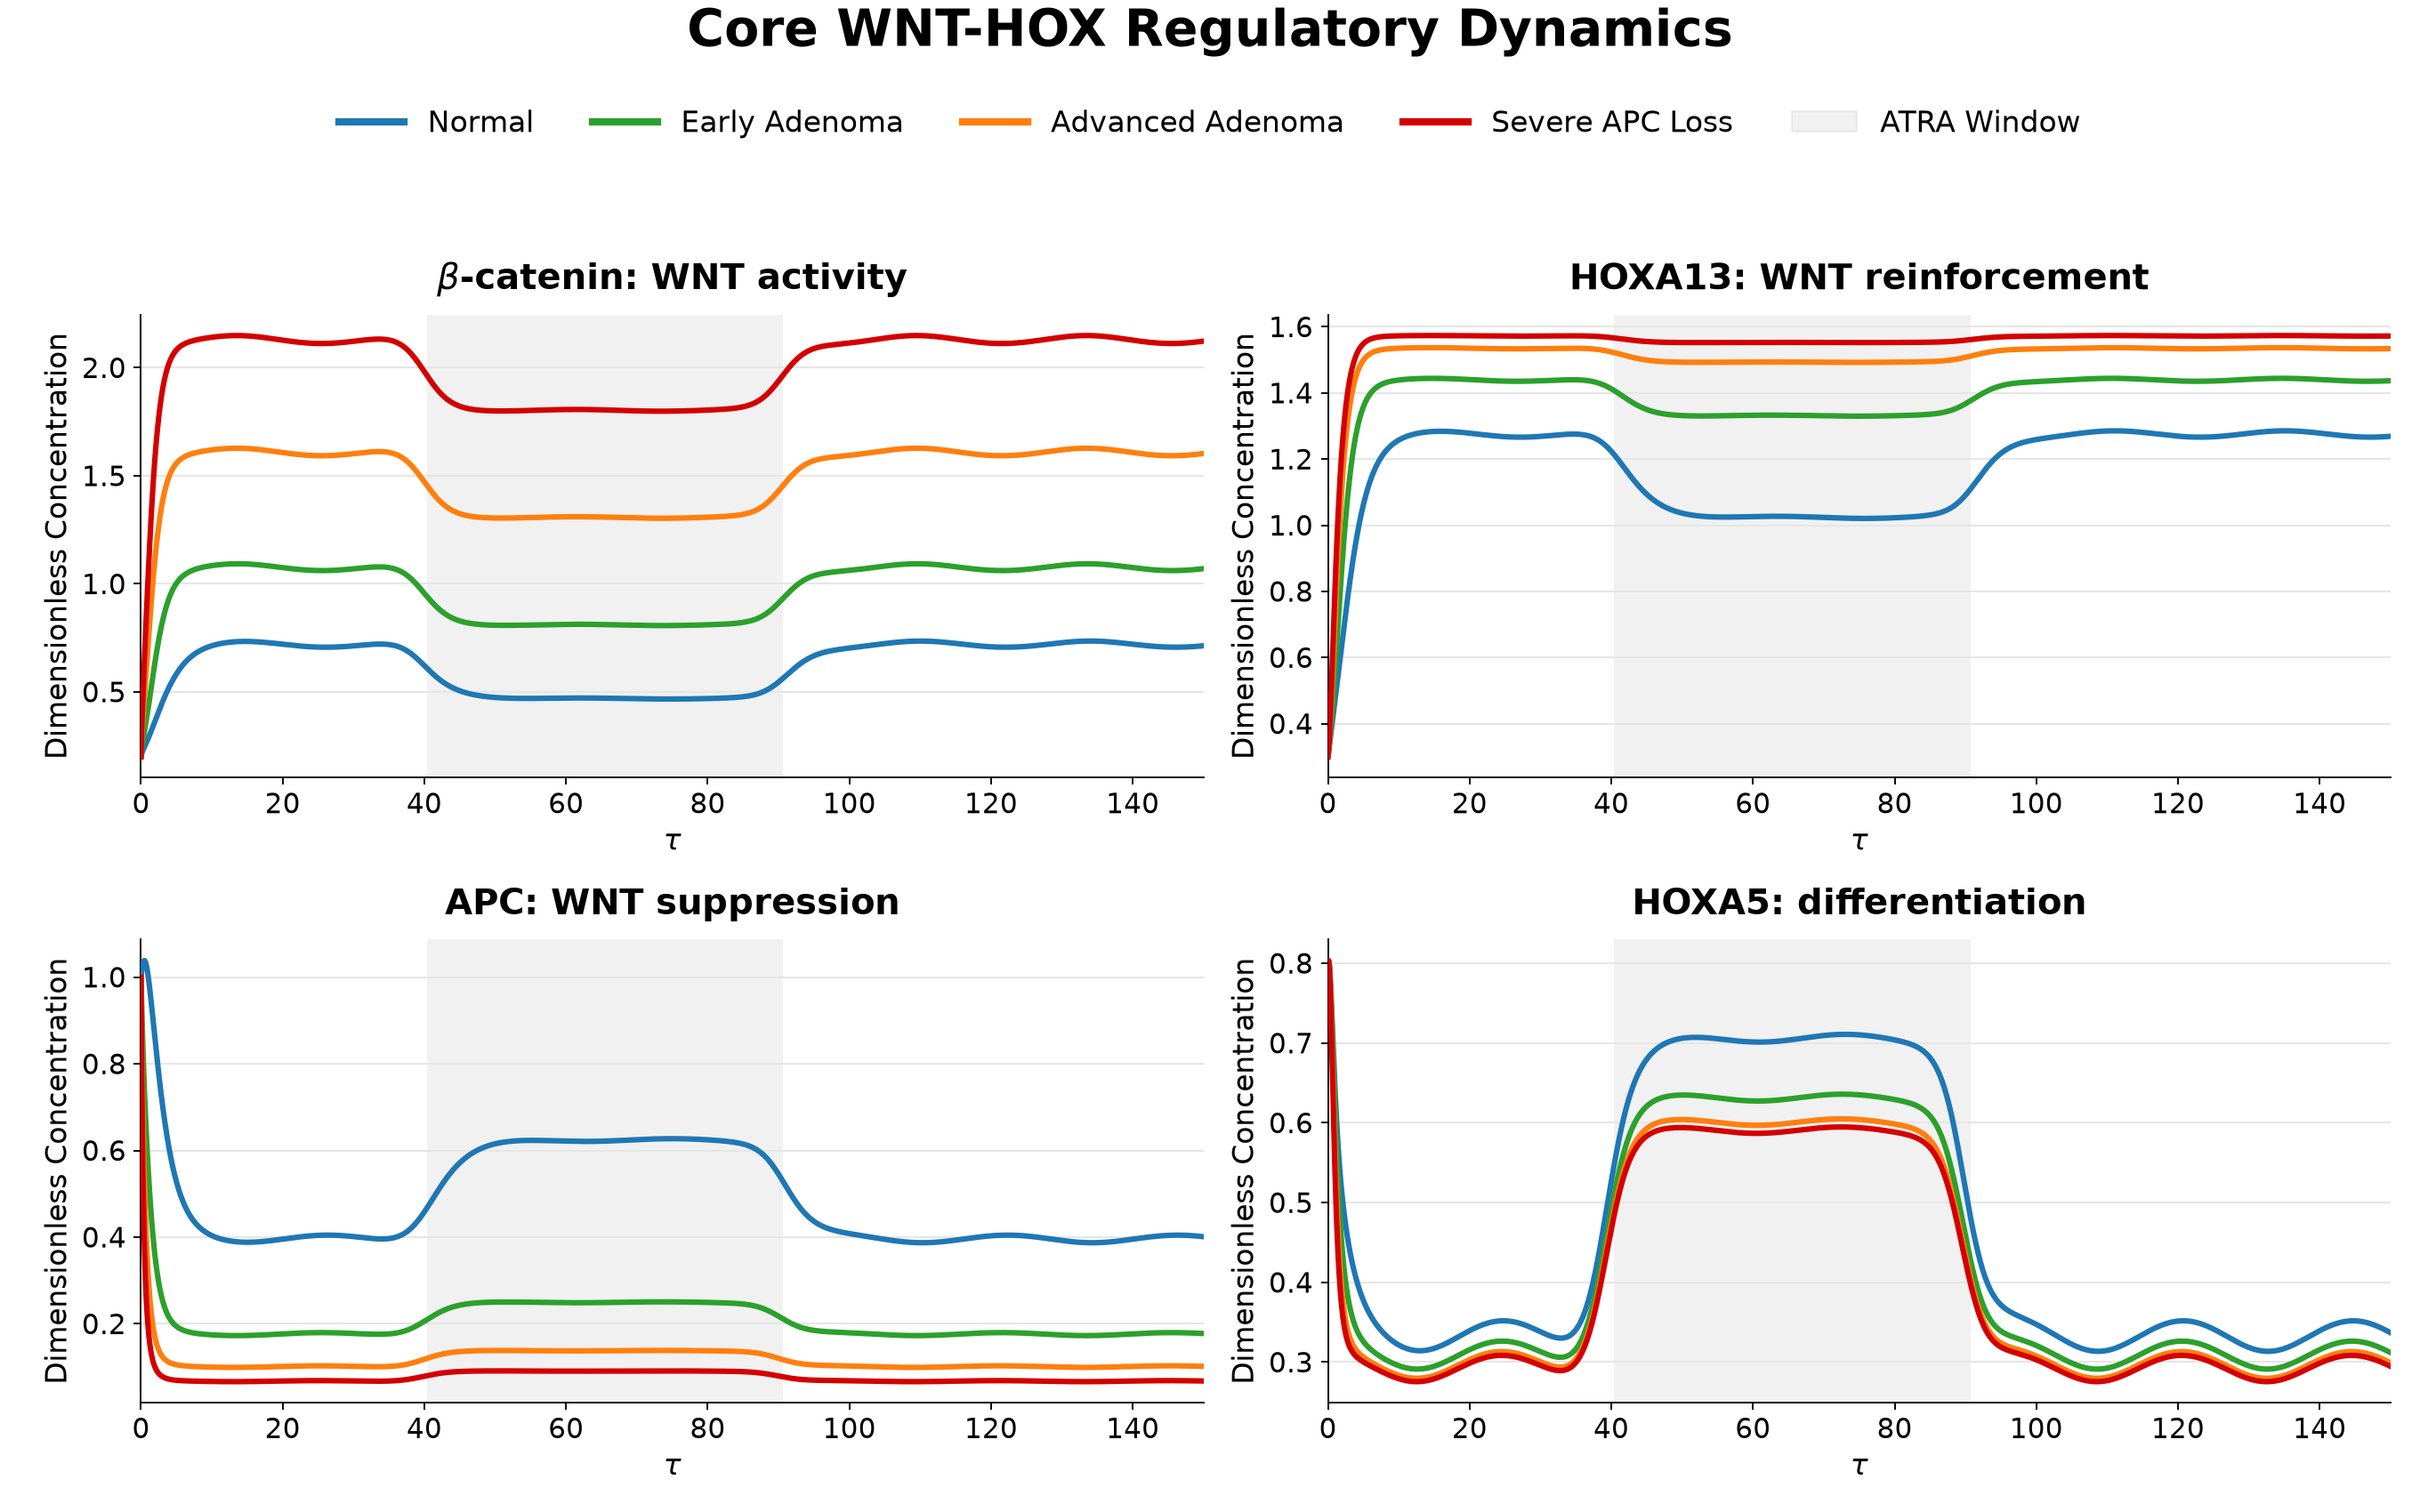
\includegraphics[width=\linewidth]{scipy.png}
    \caption{Reference trajectories of all seven states across the four
    regimes, computed with \texttt{solve\_ivp}/\texttt{Radau}. The ATRA
    treatment window is $[\tau_1,\tau_2] = [40,88]$.}
    \label{fig:scipy}
\end{figure}

The reference solutions in Figure~\ref{fig:scipy} reproduce the qualitative
behavior the model was constructed to capture. The concentrations of \bcat{}
and HOXA13 both fall during the ATRA treatment window, consistent with their
role as proliferation-associated species, and both sit at higher levels in the
more severe regimes. The HOXA13 trajectories are particularly informative: in
the Advanced Adenoma and Severe APC Loss regimes the concentration barely
decreases during treatment. The model therefore predicts that at later stages
of progression ATRA becomes ineffective at suppressing HOXA13 --- a loss of
treatment response that emerges from the network rather than being imposed.
Conversely, APC and HOXA5 rise during the treatment window, confirming their
differentiating role, and both decline as the cancer worsens. While HOXA5
responds strongly to ATRA in all four regimes, APC is markedly less responsive
at later stages, because the elevated degradation $\delta_P(\thP)$ caps the
level APC can reach regardless of how much HOXA5 is induced.

\section{Global sensitivity analysis}
\label{sec:sa}

Before asking which parameters can be \emph{recovered}, it is worth asking
which parameters \emph{matter}. A parameter to which no observable is sensitive
cannot be recovered by any method, and identifying such parameters in advance
both explains later failures and suggests a reduced model. We therefore screen
the parameter space with three complementary methods, following standard
practice in systems biology~\citep{saltelli2010variance}, and we apply the same
suite twice: to the reduced seven-state model that is the subject of this paper,
and to the full 27-state reaction network from which it descends.

\subsection{Sampling design and sensitivity measures}

All three methods score the same class of quantity of interest: the
time-averaged value of an output over the horizon,
\begin{equation}
Q[s] = \frac{1}{T}\int_0^T s(\tau)\,d\tau,
\end{equation}
evaluated for each of the seven states and for the stemness index
\eqref{eq:stemness}. Averaging rather than sampling at a point avoids making
the ranking an artifact of an arbitrarily chosen readout time.

\paragraph{Local elasticity.} The normalized local sensitivity
\begin{equation}
E_{ij} = \frac{\partial Q_i}{\partial p_j}\cdot\frac{p_j}{Q_i}
\end{equation}
is computed by central differences with a relative step of $5\%$. It is signed,
which makes it interpretable --- the sign tells you the direction of the effect
--- but it is a linearization valid only in a neighborhood of the baseline.

\paragraph{Morris elementary effects.} The Morris
screening design~\citep{morris1991factorial,campolongo2007screening} samples
one-at-a-time trajectories through a discretized parameter box and reports, for
each parameter, the mean absolute elementary effect $\mu^*$ (overall influence)
and the standard deviation $\sigma$ (evidence of nonlinearity or interaction).
The conventional flag $\sigma > \mu^*/2$ marks a parameter whose effect is
strongly nonlinear or depends on the values of others. Morris is cheap ---
$N(P+1)$ model evaluations --- and is used as a screen rather than a
quantitative decomposition.

\paragraph{Sobol variance decomposition.} The Sobol
indices~\citep{sobol2001global,saltelli2010variance} decompose the variance of
$Q$ induced by the parameter distribution into contributions from each
parameter alone ($S_1$, first order) and from each parameter including all its
interactions ($S_T$, total order). A large gap $S_T \gg S_1$ is the signature of
interaction; $\sum_j S_1^{(j)} \approx 1$ indicates a nearly additive response.
Sobol is the most informative and the most expensive of the three.

All sampling and index estimation use SALib~\citep{herman2017salib}, and every
parameter is varied within a $\pm 30\%$ box around its baseline value.

\subsection{Sensitivity of the reduced seven-state model}

For the reduced model we vary the 14 parameters that carry the regulatory
couplings and the treatment: $\thP$, $D_R$, $A_R$, $\eta_R$, $\eta_M$,
$\eta_{13}$, $\eta_{B13}$, $\eta_{BM}$, $\eta_{BC}$, $\lambda_C$, $\lambda_P$,
$\lambda_5$, $\rho_B$, $\rho_{13}$. Morris uses $N = 40$ trajectories at 4
levels (600 model solves); Sobol uses $N = 256$ base samples without
second-order indices (4096 solves). Reference trajectories are integrated with
LSODA at $\mathrm{rtol}=10^{-7}$, $\mathrm{atol}=10^{-9}$.

\paragraph{A sampling artifact, and its correction.}
One result must be reported before any other, because it invalidates part of
the naive analysis. The $\pm 30\%$ box places $\thP$ in $[0.70, 1.30]$. But the
APC degradation modifier \eqref{eq:deltaP} satisfies
\begin{equation}
\delta_P(\thP) = 1 + \delta_{P1}(1-\thP) < 0
\qquad\Longleftrightarrow\qquad
\thP > 1 + \frac{1}{\delta_{P1}} = 1.2857,
\end{equation}
for $\delta_{P1} = 3.5$. Samples with $\thP > 1.2857$ therefore give APC a
\emph{negative} decay rate and the trajectory diverges. At $\thP = 1.30$ the
time-averaged APC readout is $6.4\times10^{3}$ against a baseline of $0.473$.

The contamination is not confined to APC. Because APC appears in the
denominator of the stemness index \eqref{eq:stemness}, a diverging $p$ collapses
stemness to $0.002$ at $\thP = 1.29$, so the stemness readout is corrupted by
the same samples. In the raw output the damage is plainly visible: the Morris
$\mu^*$ for APC reaches $5.2\times10^{3}$ with $\sigma = 5.1\times10^{3}$, and
the Sobol first-order indices for APC sum to $1.145 > 1$ with
$S_1(\thP) = 1.146 \pm 1.198$ --- an impossible value for a variance share.

Since $\thP$ is a functionality fraction, $\thP > 1$ has no biological meaning
in any case, so we re-ran the entire analysis with the $\thP$ box clipped at
$1.0$. This removes the divergence: the APC first-order indices then sum to
$0.807$, and no readout is anomalous. It also, unavoidably, halves the sampled
range of $\thP$ (from $0.6$ wide to $0.3$) while leaving every other parameter
at the full $\pm 30\%$. The clipped design is therefore no longer balanced, and
$\thP$'s global scores are not on an equal footing with the others. We report
both boxes, compare \emph{rankings} rather than magnitudes across them, and
treat the clipped run as the valid one. Local elasticities, which perturb by
only $5\%$ and never leave the admissible region, are identical under both and
are unaffected throughout.

We dwell on this because the hazard is general. A proportional-perturbation box
is applied mechanically to every parameter at once, and it takes a deliberate
check to notice that one of them has a hard constraint inside the box. The
symptom here --- a variance share exceeding one --- was visible in the output,
but only because we looked; the Morris ranking that the contaminated run
produced was superficially plausible, and, as the next paragraph shows, wrong.

\paragraph{Results.} Table~\ref{tab:sa7} gives the three methods' verdicts on
the stemness index, the aggregate readout the model exists to predict.

\begin{table}[H]
\centering
\begin{tabular}{lrrrr}
\toprule
\textbf{Parameter} & \textbf{elasticity} & \textbf{Morris $\mu^*$} &
\textbf{Sobol $S_1$} & \textbf{Sobol $S_T$} \\
\midrule
$\thP$        & $-3.609$ & 0.448 & 0.154 & 0.183 \\
$\eta_{13}$   & $+1.038$ & 0.533 & 0.232 & 0.247 \\
$\eta_R$      & $-0.891$ & 0.442 & 0.167 & 0.174 \\
$\lambda_P$   & $-0.781$ & 0.288 & 0.070 & 0.072 \\
$\eta_{B13}$  & $+0.676$ & 0.371 & 0.109 & 0.115 \\
$\eta_M$      & $+0.645$ & 0.333 & 0.086 & 0.093 \\
$\lambda_5$   & $-0.512$ & 0.258 & 0.064 & 0.064 \\
$\rho_{13}$   & $+0.479$ & 0.178 & 0.021 & 0.027 \\
$\eta_{BM}$   & $+0.343$ & 0.161 & 0.016 & 0.022 \\
$\lambda_C$   & $+0.259$ & 0.123 & 0.017 & 0.016 \\
$\rho_B$      & $+0.219$ & 0.082 & 0.006 & 0.008 \\
$\eta_{BC}$   & $+0.160$ & 0.082 & 0.006 & 0.007 \\
$D_R$         & $-0.083$ & 0.041 & 0.000 & 0.002 \\
$A_R$         & $-0.037$ & 0.018 & 0.002 & 0.000 \\
\bottomrule
\end{tabular}
\caption{Sensitivity of the stemness index in the reduced model, ordered by
elasticity magnitude. Morris and Sobol columns are from the $\thP$-clipped
sampling box; elasticities are box-independent. Recall that $\thP$'s clipped
range is half the width of every other parameter's, which depresses its two
global scores relative to the rest of the column.}
\label{tab:sa7}
\end{table}

Four observations follow, one of which is a correction.

First, \textbf{APC functionality dominates the local picture}. Its elasticity on
stemness is $-3.61$, three and a half times the next largest, and the sign is
correct --- more APC function, less stemness. The same parameter has the largest
elasticity on every individual state, positive on APC ($+4.85$) and negative on
\bcat{} ($-2.01$).

Second, and this is the correction, \textbf{that dominance does not survive
into the global measures once the sampling artifact is removed}. In the
contaminated box $\thP$ towered over everything, with Morris $\mu^* = 1.212$
against $0.337$ for the runner-up and $S_1 = 0.750$ of stemness variance. In
the clipped box its Morris score falls to $0.448$, slightly \emph{below}
$\eta_{13}$ at $0.533$, and its $S_1$ falls to $0.154$, below both $\eta_{13}$
($0.232$) and $\eta_R$ ($0.167$). The overall Morris ranking across all eight
outputs likewise changes from $\thP$ alone at the top to a cluster of
$\eta_R$ ($0.509$), $\eta_{13}$ ($0.497$) and $\thP$ ($0.478$). Part of that
drop is the halved sampling range and is an artifact of the fix rather than a
finding; but the direction is unambiguous, and the honest statement is that
$\thP$ sits in a top cluster of three or four parameters globally rather than
standing alone. A conclusion drawn from the uncorrected run --- and it is the
conclusion one would naturally have drawn --- would have overstated the case.

The two pictures are not in conflict, because they answer different questions.
Local elasticity asks how strongly the output responds to a small perturbation
\emph{at the baseline operating point}, where $\thP = 1$ and the APC
degradation term is exactly at the hinge of Eq.~\eqref{eq:deltaP}. Morris and
Sobol ask how much of the output variation is attributable to a parameter
\emph{across a whole range}. A parameter can be the steepest lever locally and
still account for a modest share of variance over a box, which is precisely
$\thP$'s situation.

Third, \textbf{each state has an identifiable own-pathway driver}. The
second-largest elasticity on HOXA5 is $\eta_R$ ($+1.02$, the RA$\to$HOXA5 arm);
on HOXA13 it is $\eta_{B13}$ ($+0.61$); on MYC it is $\eta_{BM}$ ($+0.93$); on
CYP26A1 it is $\eta_{BC}$ ($+0.57$); and on RA it is $\lambda_C$ ($-0.55$) and
$D_R$ ($+0.47$), the CYP26A1 degradation arm and the treatment dose. The
network's wiring is legible in the sensitivity structure.

Fourth, and most useful for what follows, \textbf{the reduced model is
essentially additive}. For stemness in the clipped box $\sum_j S_1 = 0.950$ and
$\sum_j S_T = 1.029$: 95\% of the output variance is first-order, and the
largest gap $S_T - S_1$ over the whole table is $0.016$. Removing the divergent
samples also cleans up the Morris nonlinearity diagnostic --- in the
contaminated box 13 of 14 parameters were flagged $\sigma > \mu^*/2$, whereas in
the clipped box \emph{none} is. What looked like pervasive nonlinearity was the
divergence. This matters for the rest of the paper: when parameter recovery
fails in Section~\ref{sec:inverse}, the failure is not caused by a tangle of
high-order interactions in the reduced model.

We attach one caveat. At $N = 256$ the bootstrap confidence intervals on the
Sobol first-order indices remain wide --- $\pm 0.067$ for $\thP$ and
$\pm 0.076$ for $\eta_{13}$ --- so the top few entries are not separated with
confidence and the second-rank magnitudes should not be over-interpreted. The
broad grouping into a leading cluster, a middle band, and a negligible tail is
robust; a strict ordering within the leading cluster is not.

Figure~\ref{fig:sa7} shows the two global screens for the stemness index, and
Figure~\ref{fig:saheat} the full signed local-elasticity map from which the
own-pathway structure above is read.

\begin{figure}[H]
    \centering
    \begin{subfigure}{0.48\textwidth}
        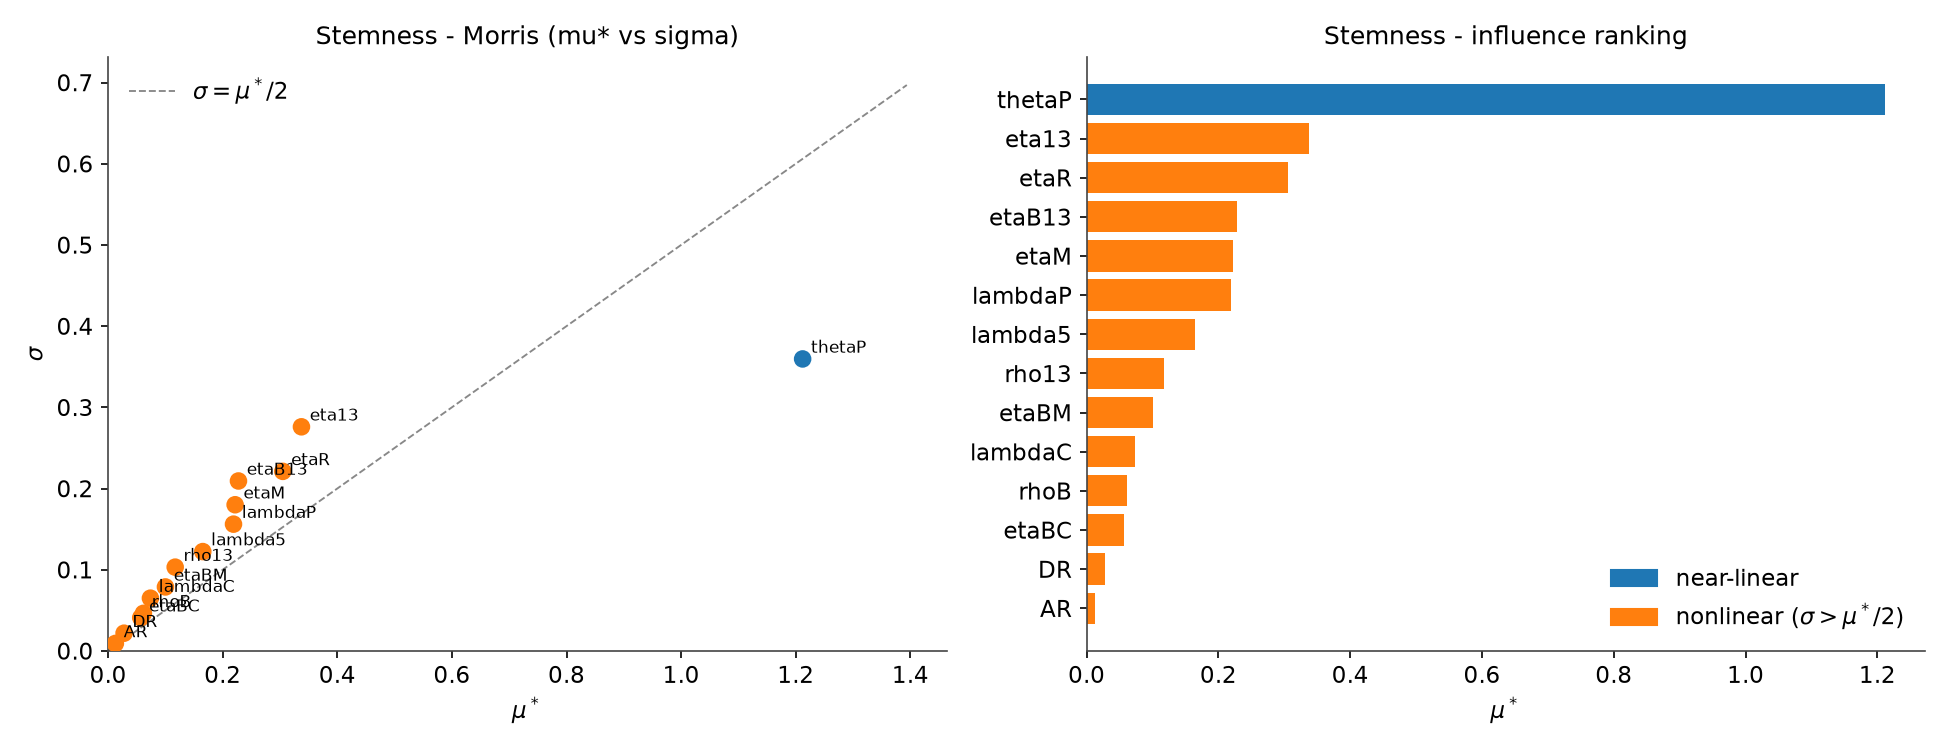
\includegraphics[width=\linewidth]{sa_morris_stemness.png}
        \caption{Morris elementary effects}
    \end{subfigure}\hfill
    \begin{subfigure}{0.48\textwidth}
        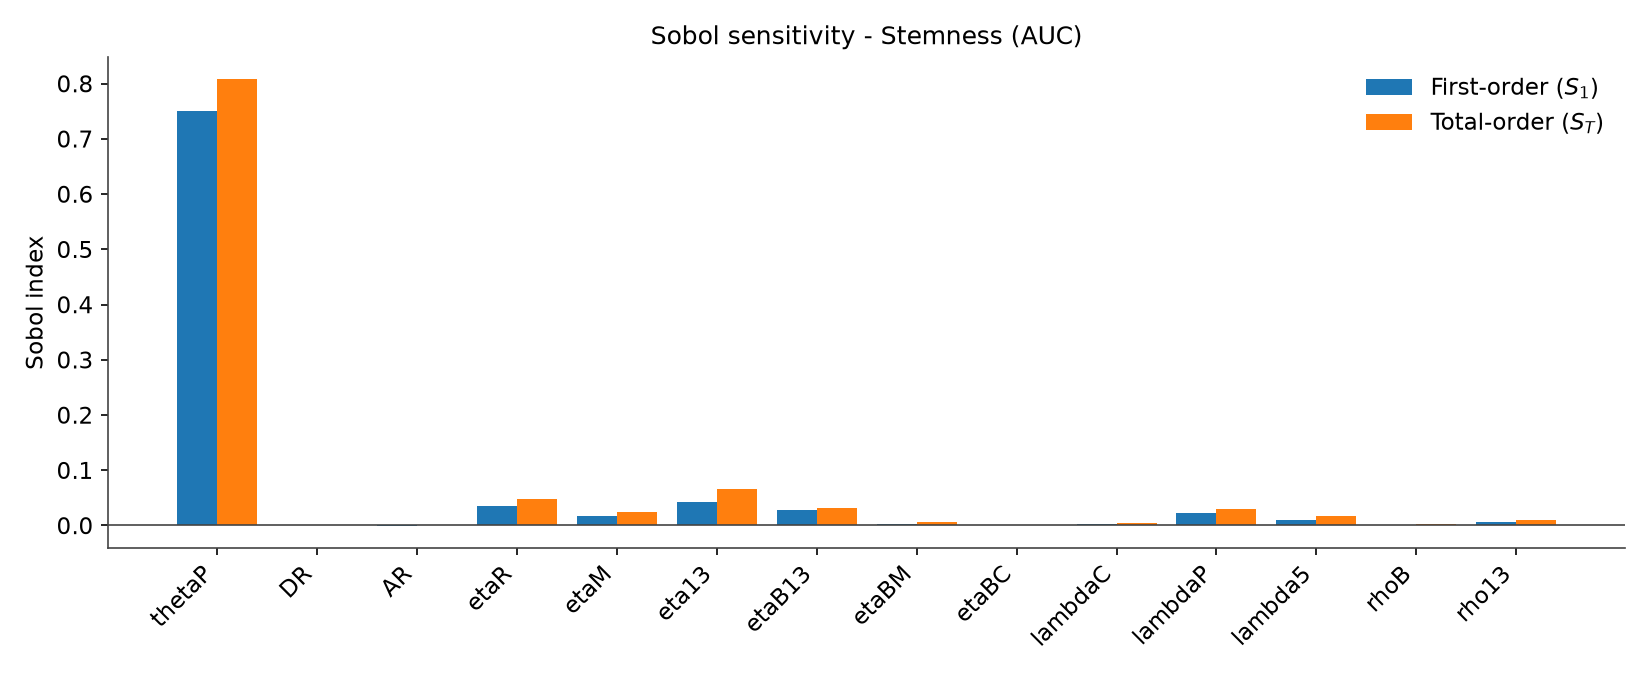
\includegraphics[width=\linewidth]{sa_sobol_stemness.png}
        \caption{Sobol indices}
    \end{subfigure}
    \caption{Sensitivity of the stemness index. The Morris panel plots $\mu^*$
    against $\sigma$ with the $\sigma = \mu^*/2$ nonlinearity line alongside the
    $\mu^*$ ranking; the Sobol panel pairs first-order and total-order indices.
    These panels are rendered from the original ($\thP$-unclipped) sampling box
    and therefore show the inflated $\thP$ bar discussed in the text; the
    corrected numbers are those of Table~\ref{tab:sa7}.}
    \label{fig:sa7}
\end{figure}

\begin{figure}[H]
    \centering
    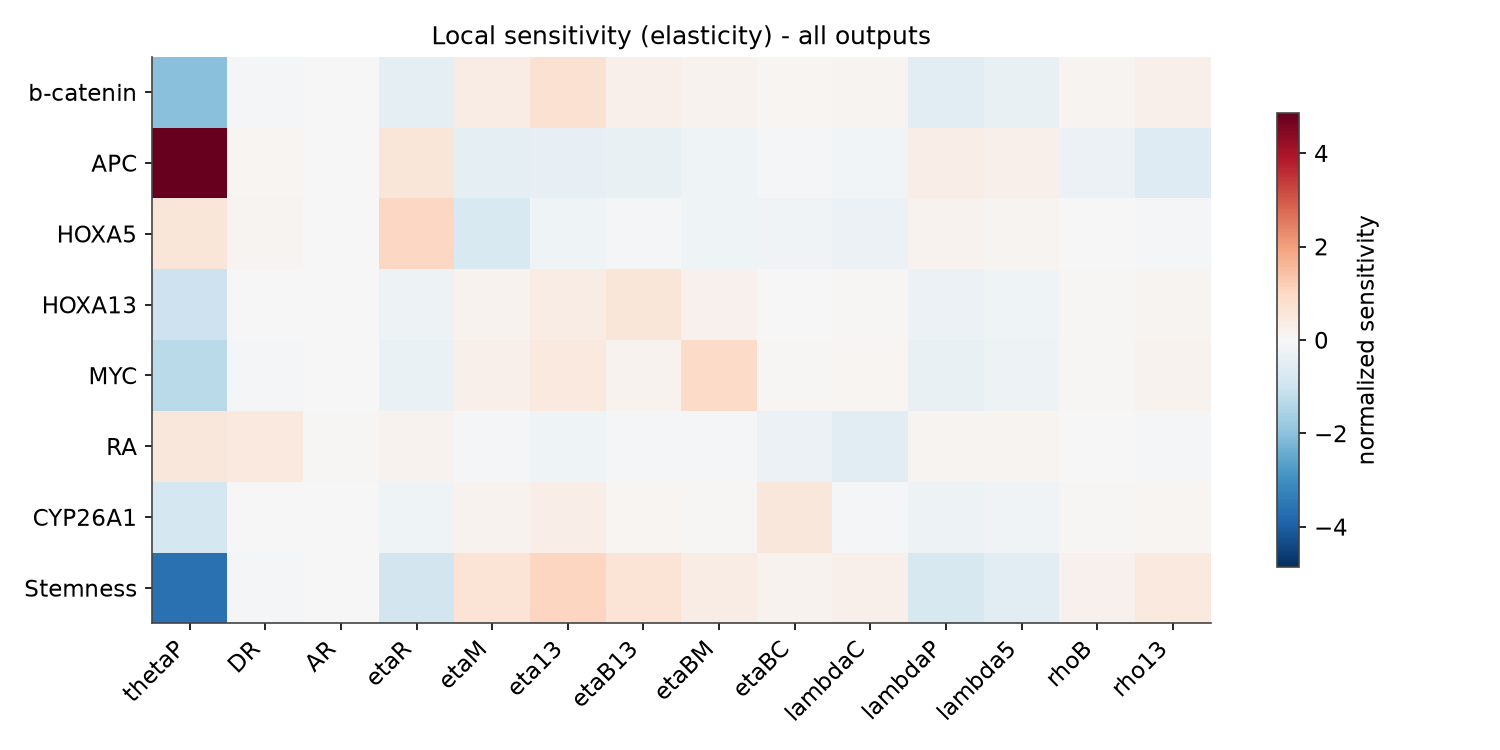
\includegraphics[width=0.85\linewidth]{sa_local_heatmap.png}
    \caption{Signed local elasticities, eight outputs by fourteen parameters.
    Blue is a positive response and red negative. The $\thP$ column dominates
    and reverses sign between the tumor-suppressor outputs (APC, HOXA5) and the
    proliferative ones (\bcat{}, HOXA13, MYC, stemness); the diagonal-like
    structure elsewhere is each output's own-pathway driver. Elasticities are
    computed with a $5\%$ perturbation and are unaffected by the sampling-box
    issue.}
    \label{fig:saheat}
\end{figure}

\subsection{Comparison with the parent 27-state network}

The reduced model is a lumping of a considerably larger reaction network: 27
states covering the retinoid block (including the binding proteins, receptors
and their complexes), the Wnt destruction-complex block, and the HOX block,
plus a derived $\beta$-catenin/TCF readout. We ran the identical three-method
suite over 30 parameters of that model --- 27 reaction rate constants plus
three cross-pathway coupling knobs --- to ask which of them the reduced model is
entitled to ignore. Solves use BDF at $\mathrm{rtol}=10^{-3}$,
$\mathrm{atol}=10^{-6}$, with outputs scored as time averages over a settled
window, and the stemness surrogate defined analogously to
Eq.~\eqref{eq:stemness}.

The consolidation rule is deliberately conservative: a parameter is a candidate
to be \emph{fixed} only if all three methods independently score it below 5\% of
that method's maximum. Anything else is \emph{kept}. The verdict is \textbf{22
keep, 8 fix}, with the fixable set $\{v_{17}, k_{15}, k_{22}, k_{p4}, k_{m1},
k_{p9}, k_{m4}, k_{m3}\}$ and the most influential parameters being
$\mathrm{MCsynth}$ (consensus score 0.999), $v_{16}$ (0.830), $k_{p5}$ (0.612),
$\gamma_1$ (0.527), $k_{p6}$ (0.464), $k_{14}$ (0.408) and $k_8$ (0.351). The
conservatism of the rule is visible in the near-ties: $v_{17}$ (consensus
0.0341) is fixed while $k_{23}$ (0.0329) is kept, because $k_{23}$ clears the
5\% bar under Morris even though its Sobol index is negligible. The full ranking
and the threshold that separates the two groups are given in
Figure~\ref{fig:sabig}.

\begin{figure}[H]
    \centering
    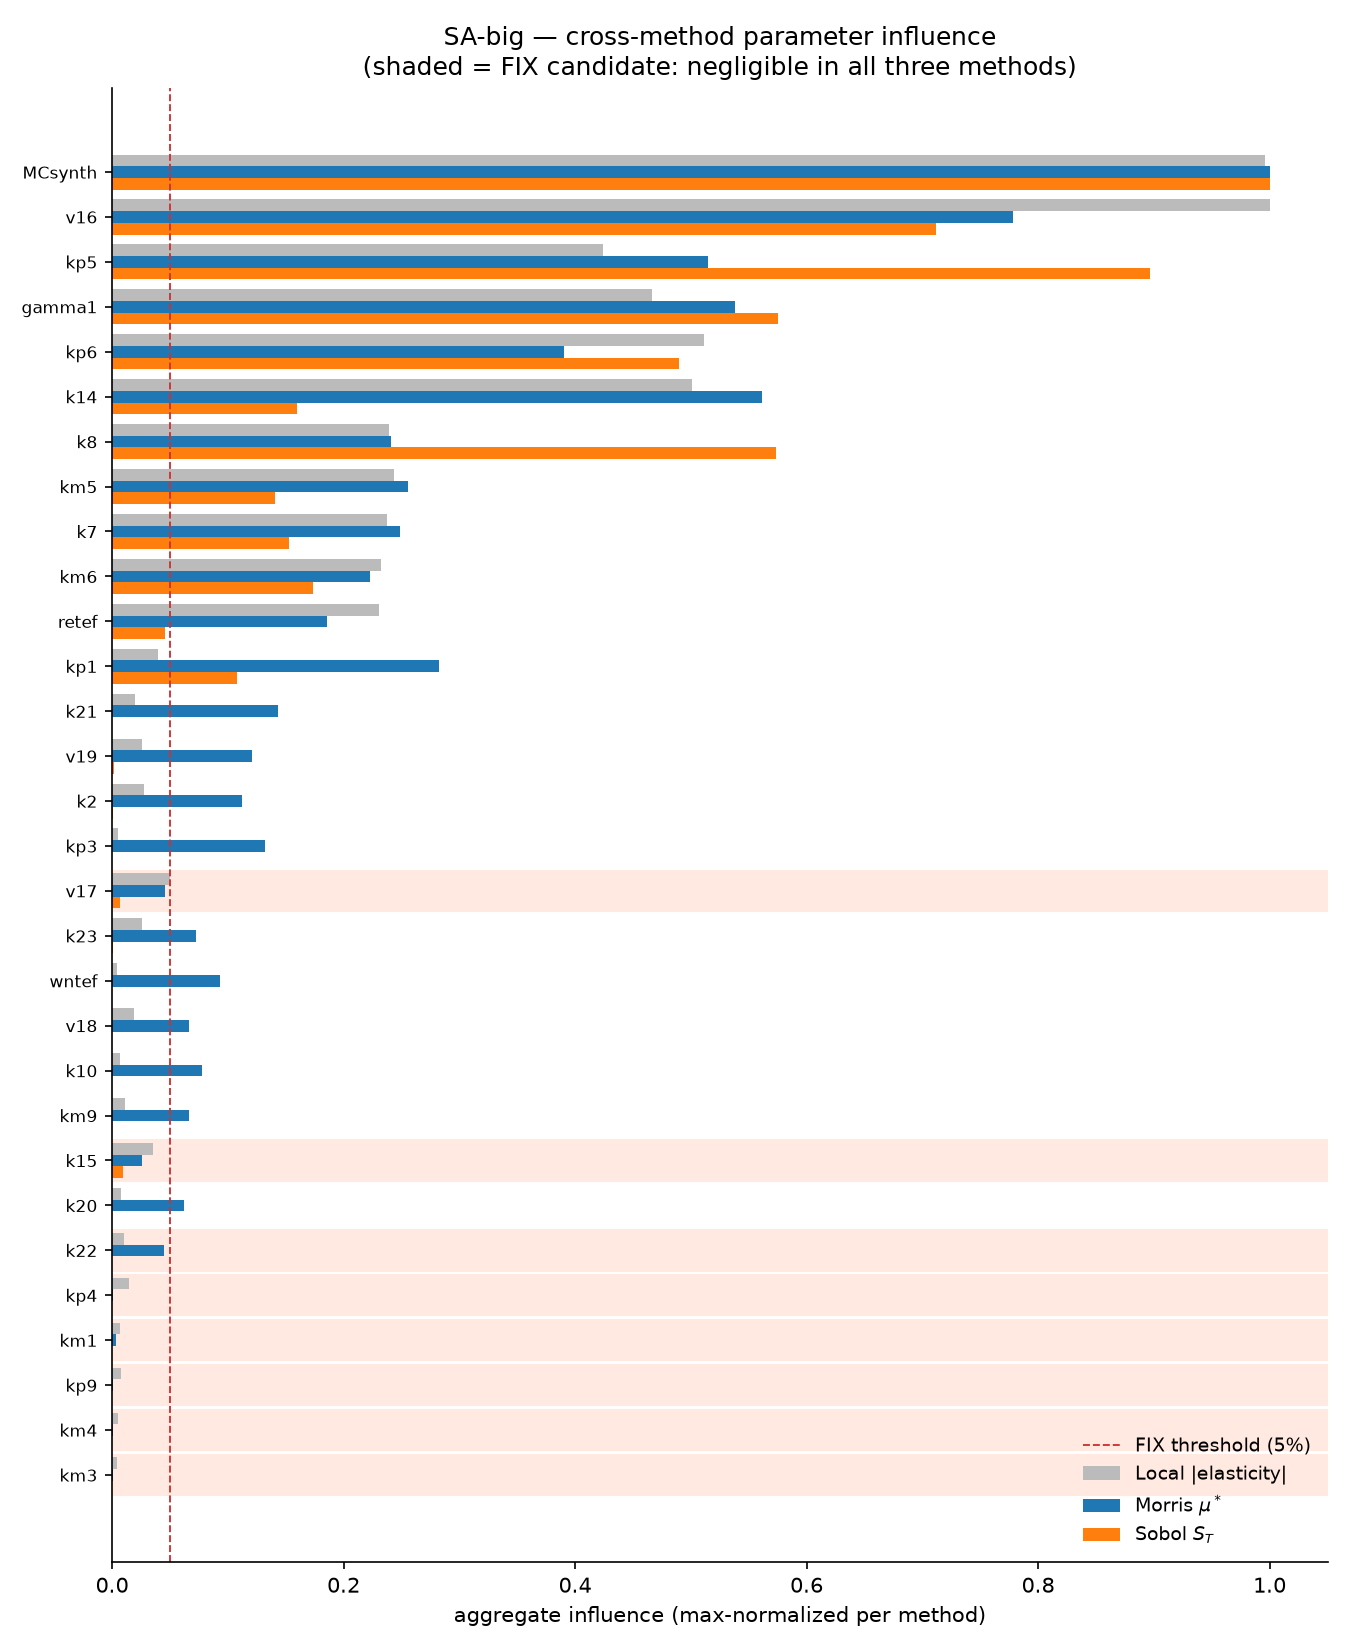
\includegraphics[width=0.9\linewidth]{sa_big_combined_ranking.png}
    \caption{Cross-method consensus ranking for the 27-state model. Bars give
    each parameter's max-normalized score under local elasticity, Morris
    $\mu^*$, and Sobol $S_T$; the dashed line is the 5\% threshold and the
    shaded rows are the eight parameters that fall below it under all three
    methods.}
    \label{fig:sabig}
\end{figure}

The instructive contrast with the reduced model is in the interaction
structure. Where the reduced model is nearly additive, the 27-state model is
strongly interacting: $\sum_j S_T$ runs from 1.9 to 4.9 against $\sum_j S_1$ of
0.6 to 1.5. For the stemness surrogate, $k_8$ has $S_1 = -0.173$ but
$S_T = 0.429$, and $k_{p5}$ moves from $S_1 = 0.156$ to $S_T = 0.502$; a
negative first-order index with a large total index is the textbook signature of
a parameter that acts purely through interactions. The single clean exception is
$\gamma_1$, the knob scaling $\beta$-catenin/TCF availability, which is almost
purely additive ($S_1 \approx S_T \approx 0.73$--$0.80$ on MYC, HOXA5, and the
$\beta$-catenin/TCF readout). Lumping the network down to seven states, in
other words, does not merely reduce dimension --- it removes most of the
interaction structure, which is part of why the reduced model is a tractable
inference target at all.

Three limitations of the 27-state analysis should be recorded. Roughly 7.5\% of
Morris solves and 8.5\% of Sobol solves failed to converge and were
mean-imputed. The Morris nonlinearity flag $\sigma > \mu^*/2$ fires for 27 to 30
of 30 parameters on every output, so at this sample size it is saturated and
carries no discriminating information --- we report it as a limitation, not a
finding. And the Sobol indices for the CYP26A1 readout are numerically
meaningless because its baseline settles to $7.6\times10^{-6}$, so the variance
ratio's denominator collapses; that row is excluded.

\subsection{Scope and limitations of the sensitivity analysis}

The screen establishes that the model's outputs are strongly and
interpretably sensitive to a modest number of parameters, and it identifies
which. It is tempting to conclude that these are the parameters an inverse
method will recover. That conclusion is wrong, and it is worth flagging here
because Section~\ref{sec:inverse} will demonstrate it directly:
\emph{a-priori sensitivity does not predict recoverability}. The clearest case
is $\eta_{BM}$, the \bcat{}$\to$MYC arm, which has the single largest relative
sensitivity of any parameter in the residual and yet recovers with a mean error
of 29\% and is judged non-recoverable overall. Conversely, several timescale
parameters sit near the bottom of the sensitivity ranking and recover to within
10--20\%. Sensitivity tells you whether a parameter can influence the data;
identifiability tells you whether its influence can be \emph{distinguished from
that of the other parameters}, and it is the second question that governs
recovery.
\section{The forward problem: neural approximation of the model trajectories}
\label{sec:forward}

The forward problem is to produce $y(\tau)$ on $[0,T]$ given the parameters.
A stiff solver already does this to machine precision, so a PINN is not
competitive as a solver here and we do not claim it is. The purpose of the
forward study is different and twofold. It establishes that a network of this
architecture can represent this system's dynamics at all --- a prerequisite for
the inverse problem, where the same networks carry the state representation ---
and it isolates the one architectural choice that the system genuinely forces.

\subsection{Network architecture and time embedding}

The state representation is a multilayer perceptron $z_\phi : \tau \mapsto
\mathbb{R}^7$ of width 256 and depth 4 with GELU activations, Xavier-normal
initialization at gain $0.5$, and 207,879 parameters. Time is not fed to the
network directly. It passes through a fixed random Fourier
embedding~\citep{tancik2020fourier},
\begin{equation}
\gamma(\tau) = \Big[\tfrac{\tau}{T},\
\sin\!\big(2\pi\tfrac{\tau}{T}B_k\big),\
\cos\!\big(2\pi\tfrac{\tau}{T}B_k\big)\Big]_{k=1}^{16},
\qquad B_k \sim \mathcal{N}(0, \sigma_F^2),\ \sigma_F = 4,
\label{eq:fourier}
\end{equation}
giving an input of dimension $1 + 2\times16 = 33$. The frequencies $B_k$ are
drawn once and held fixed as a buffer, not trained. Retaining the raw
normalized time $\tau/T$ alongside the sinusoids lets the network represent the
slow trend and satisfy the initial condition without having to synthesize them
from oscillatory components.

The scale $\sigma_F$ is the one hyperparameter that must be matched to the
problem. The circadian forcing has period $T_R = 24$ over a horizon of $T=150$,
so representing it requires a frequency near $150/24 = 6.25$ in the units of
Eq.~\eqref{eq:fourier}. The realized draw contains three frequencies that
bracket this value ($6.94$, $-6.99$, $-7.16$), with the remainder spread over
$|B_k| \in [0.69, 7.16]$, i.e. implied periods from $21$ to $216$ time units.
Sixteen features at $\sigma_F = 4$ therefore span both the treatment pulse and
the circadian ripple, which is why this configuration suffices.

\subsection{Composite loss and training protocol}

We report two variants. The \emph{dense-label baseline} fits 100 evenly spaced
labeled points with loss weights $\lambda_{\text{data}} = 0.7$,
$\lambda_{\text{phys}} = 0.3$ and no explicit initial-condition term; it is a
supervised interpolation of a pre-solved trajectory, included as a reference
point. The \emph{sparse hybrid} is the honest forward solve and is the variant
we emphasize: it sees only 40 observations drawn uniformly at random from the
horizon and must reconstruct everything between them from the physics. Its
objective is
\begin{equation}
\mathcal{L} = \lambda_{\text{data}}\mathcal{L}_d
+ \lambda_{\text{phys}}\mathcal{L}_p
+ \lambda_{\text{ic}}\mathcal{L}_{\text{ic}},
\qquad
\lambda_{\text{data}} = \lambda_{\text{phys}} = 1,\quad
\lambda_{\text{ic}} = 20,
\label{eq:fwdloss}
\end{equation}
with
\begin{equation}
\mathcal{L}_d = \frac{1}{N_d}\sum_{i}\big\|z_\phi(\tau_i) - y_i\big\|^2,
\qquad
\mathcal{L}_p = \frac{1}{N_c}\sum_{k}
\Big\|\dot z_\phi(\tau_k) - f\big(\tau_k, z_\phi(\tau_k);\theta\big)\Big\|^2,
\qquad
\mathcal{L}_{\text{ic}} = \big\|z_\phi(0) - y_0\big\|^2 .
\end{equation}
The initial condition is imposed as a weighted penalty rather than hard-wired
into an ansatz. The derivative $\dot z_\phi$ is taken by automatic
differentiation; this is unremarkable in the forward problem, where the
parameters are known, but it becomes the central issue in
Section~\ref{sec:inverse}. Collocation uses $N_c = 50{,}000$ points resampled
uniformly at random every epoch, reduced to $10{,}000$ during the L-BFGS phase.

The realized sparse design (seed 42) places observations with a median gap of
$2.76$ and a maximum gap of $13.92$ time units, giving about 6.4 observations
per circadian period, with 13 of the 40 falling inside the treatment window.
This is a genuinely sparse and irregular design: several circadian cycles are
covered by fewer than two points, so the oscillation between them is supplied
by the physics residual, not by interpolation.

Training is two-stage: Adam~\citep{kingma2015adam} for 1000 epochs at learning
rate $10^{-3}$ with cosine annealing to $10^{-6}$, followed by 500 outer steps
of L-BFGS~\citep{liu1989lbfgs} with strong-Wolfe line search, history size 50
and up to 20 inner iterations per step. All computation is in float64.

\subsection{Accuracy against the reference solution}

Table~\ref{tab:fwderr} reports the error of the trained networks against the
Radau reference on a uniform grid of 6000 points spanning the full horizon. We
give both relative $L^2$ error and NRMSE (RMSE normalized by the range of the
reference), for a reason visible in the table: APC settles to a very small
value in the high-WNT regimes, so its relative $L^2$ error is inflated by a
vanishing denominator. In Severe APC Loss the APC relative $L^2$ is $13.53\%$
while its NRMSE is $1.26\%$, entirely in line with every other state. NRMSE is
the fair summary for that species.

\begin{table}[H]
\centering
\small
\setlength{\tabcolsep}{4pt}
\begin{tabular}{lrrrrrrrrr}
\toprule
\textbf{Regime} & \bcat{} & APC & HOXA5 & HOXA13 & MYC & RA & CYP26A1 &
\textbf{mean} & \textbf{NRMSE} \\
\midrule
\multicolumn{10}{l}{\emph{Sparse hybrid, 40 random observations + IC + physics}}\\
Normal            & 2.93 & 5.85  & 1.79 & 2.93 & 2.69 & 1.71 & 1.93 & 2.83 & 2.86 \\
Early Adenoma     & 1.56 & 2.84  & 1.61 & 1.80 & 1.59 & 1.74 & 1.16 & 1.76 & 1.51 \\
Advanced Adenoma  & 0.91 & 7.02  & 1.69 & 1.33 & 1.02 & 1.75 & 0.89 & 2.09 & 1.20 \\
Severe APC Loss   & 0.86 & 13.53 & 1.94 & 1.18 & 0.86 & 1.49 & 0.81 & 2.95 & 1.16 \\
\midrule
\multicolumn{10}{l}{\emph{Dense-label baseline, 100 evenly spaced labels}}\\
Normal            & 0.39 & 0.74 & 0.70 & 0.21 & 0.25 & 0.73 & 0.38 & 0.49 & 0.46 \\
Early Adenoma     & 0.34 & 1.27 & 0.95 & 0.25 & 0.41 & 1.00 & 0.34 & 0.65 & 0.49 \\
Advanced Adenoma  & 0.27 & 4.14 & 1.43 & 0.36 & 0.56 & 1.06 & 0.37 & 1.17 & 0.62 \\
Severe APC Loss   & 0.36 & 9.11 & 1.41 & 0.34 & 0.55 & 1.26 & 0.37 & 1.91 & 0.68 \\
\bottomrule
\end{tabular}
\caption{Forward PINN accuracy: per-state relative $L^2$ error (\%) against the
\texttt{Radau} reference over $\tau \in [0,150]$, with the per-regime mean and
mean NRMSE (\%) in the last two columns. Grand means: sparse hybrid $2.41\%$
relative $L^2$ ($1.59\%$ excluding APC), $1.68\%$ NRMSE; dense baseline
$1.06\%$ relative $L^2$, $0.56\%$ NRMSE.}
\label{tab:fwderr}
\end{table}

The headline comparison is the one the two halves of the table invite. The
sparse hybrid reaches $2.41\%$ mean relative $L^2$ from 40 randomly placed
observations, against $1.06\%$ for the dense baseline from 100 evenly spaced
ones. Reconstructing the full seven-state trajectory to within roughly $2.4\times$
the dense-label error, from $2.5\times$ fewer and irregularly spaced points, is
what the physics term buys: the residual constrains the solution everywhere on
the horizon, including across the wide gaps where no data exist. We reproduced
this comparison in two independent runs a month apart with essentially
identical results (sparse-hybrid per-regime means of $2.90/1.71/2.24/2.96$ in
the earlier run), so the figures are stable under rerun, though every run uses
the same seed and we therefore have no estimate of seed-to-seed variability.

The composition of the final loss is worth noting as a diagnostic. In the
sparse hybrid the physics term accounts for 94--97\% of the total loss at the
end of Adam training; the data term is essentially satisfied early and the
optimizer spends the remainder of its budget enforcing the ODE. In the dense
baseline the two terms remain the same order of magnitude throughout. This is
the expected signature of a genuinely physics-driven solve versus a
data-driven one. Figure~\ref{fig:forwardpinn} shows the reconstruction itself
for the four core WNT--HOX species.

\begin{figure}[H]
    \centering
    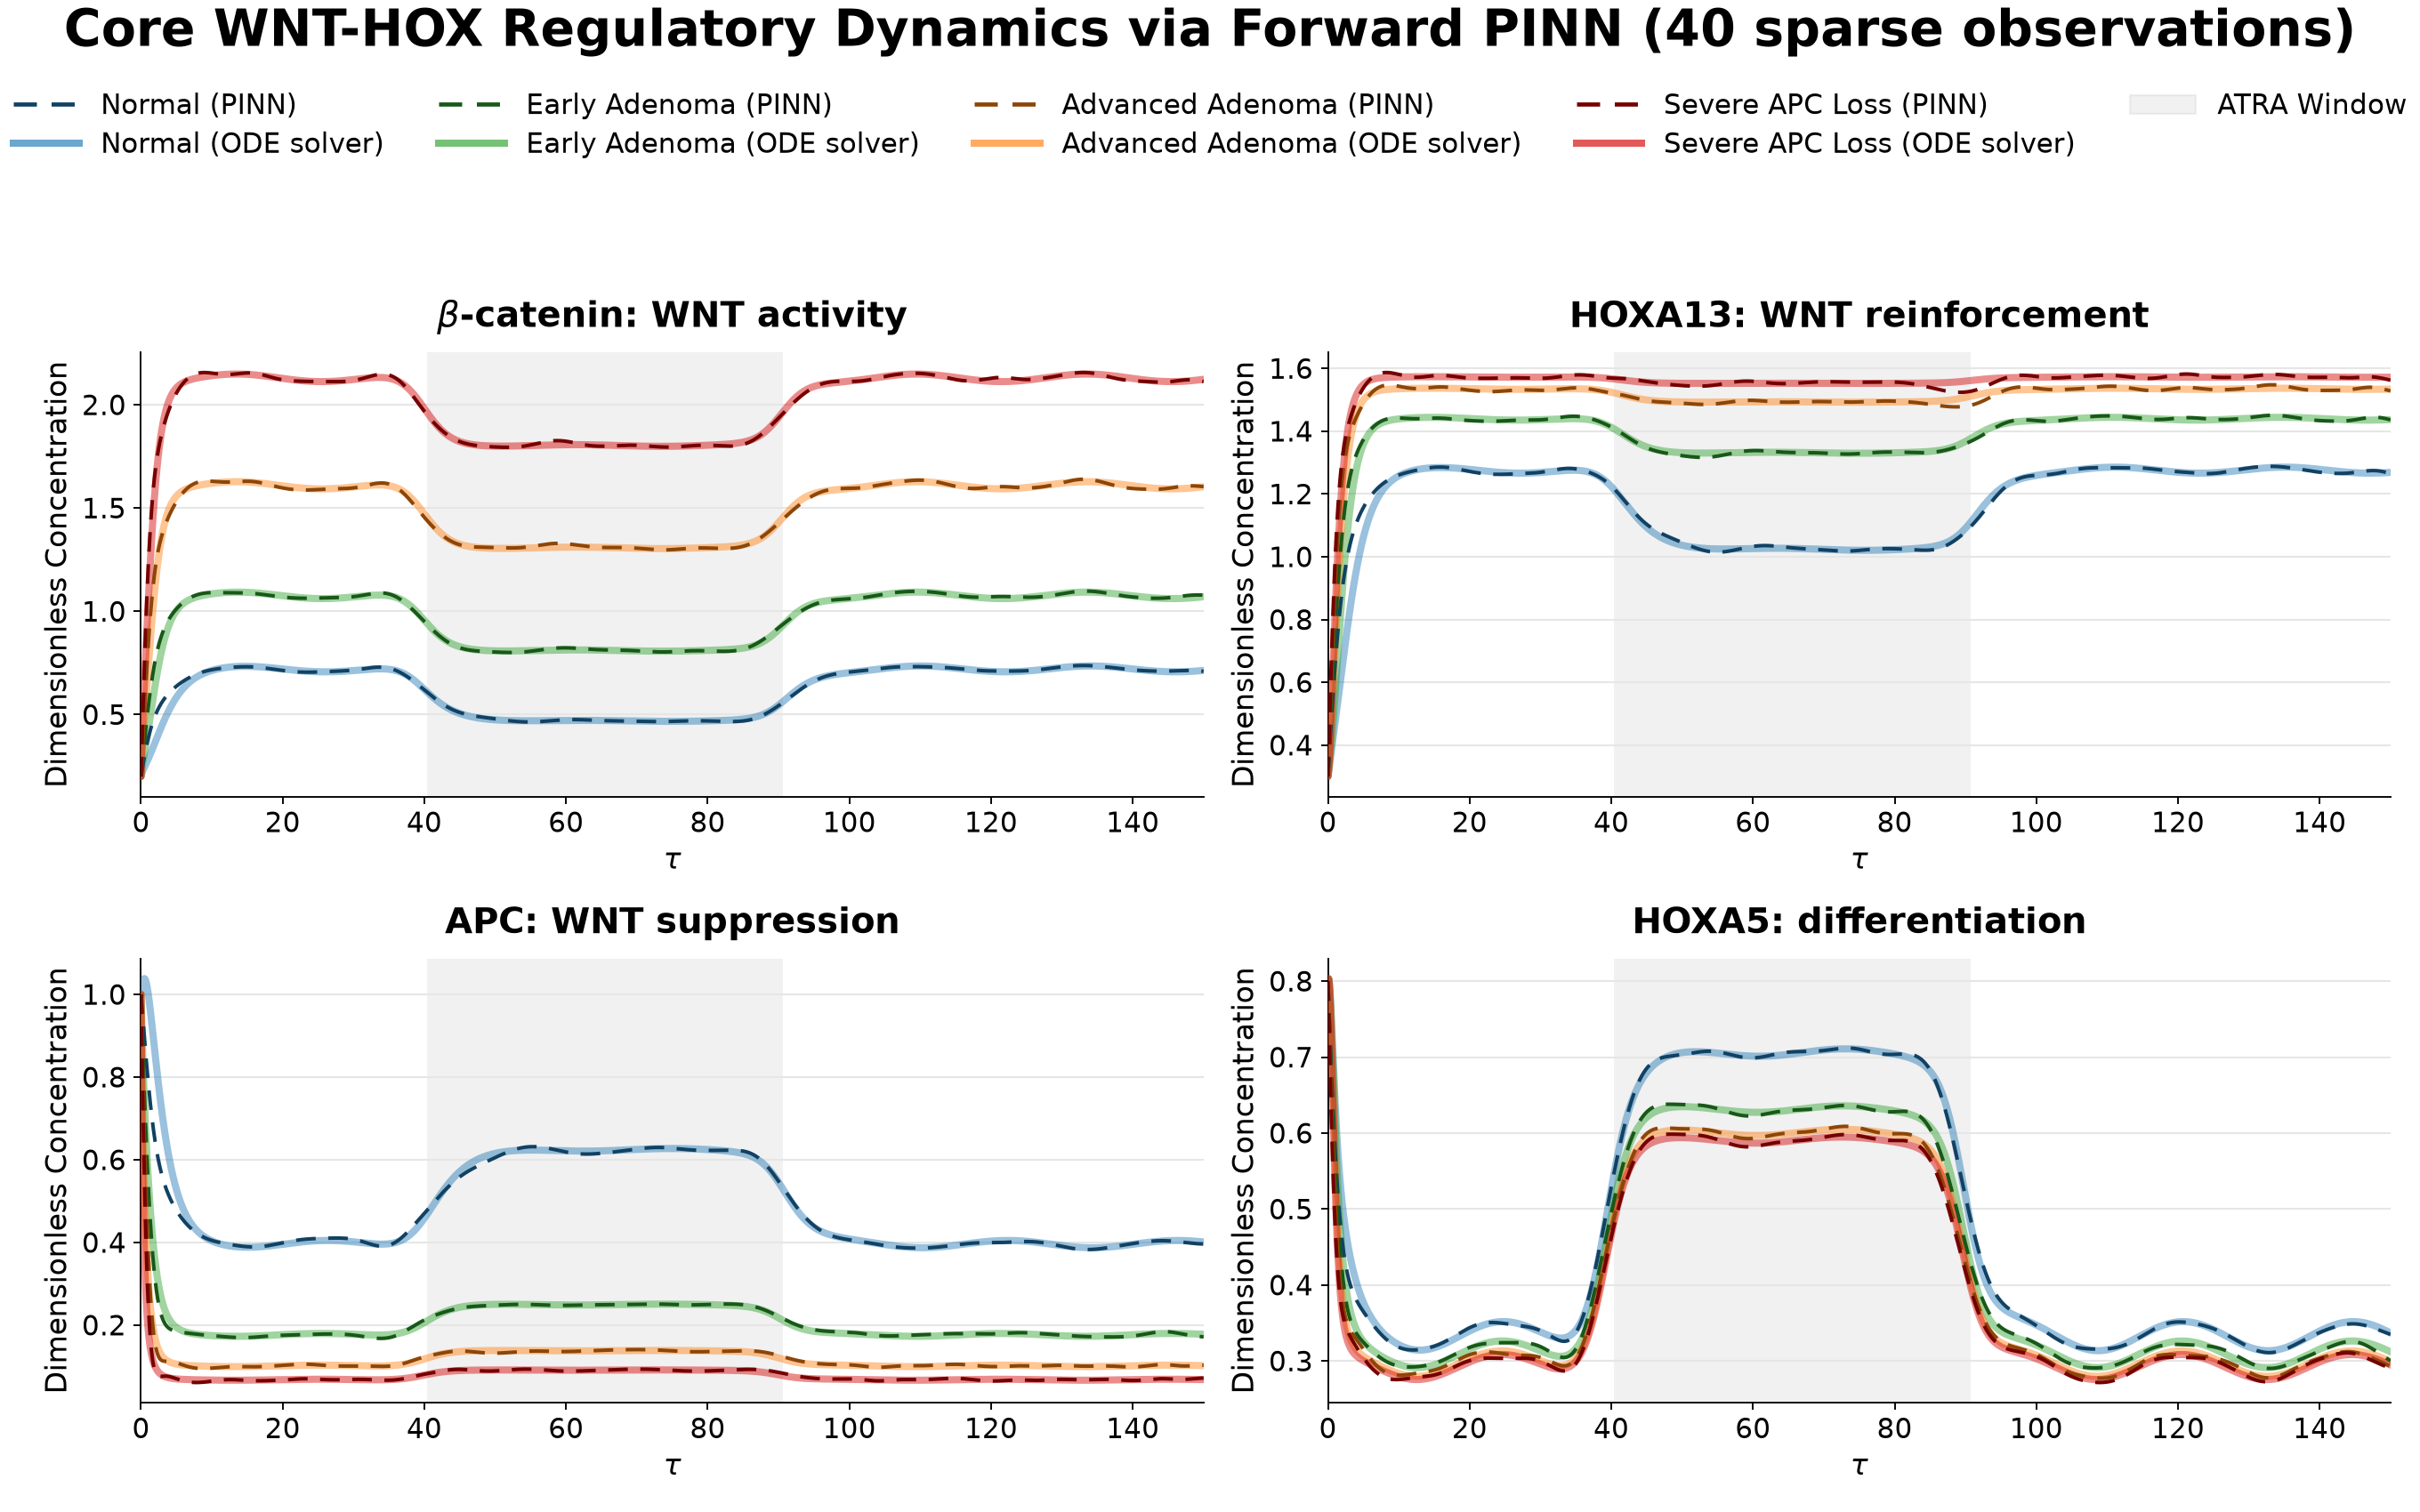
\includegraphics[width=\linewidth]{forward_pinn_hybrid.png}
    \caption{Forward PINN reconstruction of the four core WNT--HOX species
    across all four regimes, from the \emph{sparse hybrid} model --- 40 random
    observations plus the physics residual. Thick translucent curves are the
    \texttt{Radau} reference and thin dashed curves the PINN. They are visually
    indistinguishable over almost the whole horizon; the one place the
    discrepancy is apparent to the eye is the steep initial transient
    ($\tau \lesssim 5$), where APC falls from $1.0$ and HOXA13 rises from
    $0.3$ faster than the network tracks. That transient is the largest
    contributor to the Normal regime's error in Table~\ref{tab:fwderr}, and it
    is where the observation design is thinnest. The shaded band is the
    \emph{half-response window} --- the median 50\% crossing of the switch-on
    and switch-off transitions across states and regimes --- which sits at
    $[40.4, 90.7]$, lagged relative to the dose window $[40,88]$ because the
    states respond with delay.}
    \label{fig:forwardpinn}
\end{figure}

\subsection{Spectral bias and the necessity of the Fourier embedding}

The Fourier embedding is not a refinement; without it the model does not solve
the problem. A plain MLP taking $\tau$ directly as a scalar input (199,687
parameters, otherwise identically trained) plateaus early and never recovers.
Its data loss stalls at $1.41\times10^{-3}$ and its physics loss at
$1.83\times10^{-2}$ by around epoch 2000 and does not improve thereafter; 500
subsequent L-BFGS steps move the total loss from $6.48\times10^{-3}$ to
$6.54\times10^{-3}$, that is, not at all. The Fourier-embedded network reaches a
data loss of $1.9\times10^{-5}$, roughly 75 times lower.

The failure is specifically a failure to represent the fast component, exactly
as spectral-bias theory predicts~\citep{rahaman2019spectral,wang2022ntk}. In the
Normal regime the plain network's RA output spans $[0.161, 0.440]$ where the
true RA spans $[0.156, 0.787]$: it captures under half the amplitude of the
ATRA pulse and none of the circadian ripple, having settled on a smooth curve
through the middle of the oscillation. The Fourier-embedded network on the same
regime spans $[0.1563, 0.7868]$ against a true $[0.1562, 0.7867]$, agreeing to
three or four decimal places. Restricted to the active window, the plain
network's mean relative $L^2$ error is 23--26\% across the four regimes.

We must disclose a confound: the surviving plain-MLP run was trained over a
horizon of $T = 3000$ rather than $T = 150$, so the embedding and the horizon
differ simultaneously and this is not a controlled ablation. The direction and
magnitude of the effect are unambiguous and consistent with the established
theory, but a clean single-variable ablation at fixed $T$ was not run and we do
not claim one.

\subsection{Summary of the forward results}

The forward study supports a narrow but necessary claim. A Fourier-feature
network of this size represents the seven-state system across all four regimes
to roughly 1--3\% error, and does so from 40 sparse observations by leaning on
the physics residual. The multi-timescale forcing makes the time embedding
mandatory rather than optional. Both facts carry directly into the inverse
problem, where the same architecture supplies the state representation and the
question shifts from whether the trajectory can be represented to whether the
parameters that generated it can be recovered.
\section{The inverse problem: parameter estimation from trajectory data}
\label{sec:inverse}

\subsection{Problem formulation and scoring criterion}

The inverse problem is to recover $\theta \in \mathbb{R}^{36}$ from sparse noisy
observations of the trajectory. In the PINN formulation the parameters become
trainable variables optimized jointly with the state
networks~\citep{raissi2019pinn}, and the objective is Eq.~\eqref{eq:fwdloss}
with $\theta$ now free. Three design decisions apply throughout.

\emph{Multiple conditions, shared parameters.} We train one state network per
experimental condition but a single shared parameter vector, so $\theta$ must
satisfy the residual under all conditions simultaneously. This is the
mechanism by which additional experiments constrain the parameters rather than
merely adding degrees of freedom.

\emph{Log parameterization.} Every positive parameter is represented as
$\theta_j = \theta_j^{\text{nom}}\exp(s_j)$ with $s_j$ trainable, and $\thP$ as
$\mathrm{sigmoid}(s)$ mapped into $(0,1)$. This enforces positivity by
construction and, more importantly, makes the gradient with respect to $s_j$ a
\emph{relative} sensitivity, so parameters whose true values differ by two
orders of magnitude receive comparably scaled updates.

\emph{Honest initialization.} All estimates start at $1.5\times$ the true value,
with $W$ and $\thP$ additionally displaced to deliberately wrong values. No
optimization is ever started at or near the truth.

We score recovery as the number of the 36 parameters whose estimate falls
within 10\% relative error, reported per regime. This threshold is a
convention, not a claim about what precision biology requires; we use it
consistently so that comparisons between methods are meaningful, and we report
per-regime counts rather than a pooled figure because the regimes differ
sharply in difficulty.

\subsection{A two-parameter proof of concept}

We first restricted the unknowns to $(W, \thP)$, the two parameters that define
the regimes. From a single condition with 80 observations at 1\% noise, the
result already contains the entire subsequent story in miniature
(Table~\ref{tab:twoparam}).

\begin{table}[H]
\centering
\begin{tabular}{lcccc}
\toprule
\textbf{Regime} & $W$ \textbf{true} & $W$ \textbf{error} &
$\thP$ \textbf{true} & $\thP$ \textbf{error} \\
\midrule
Normal            & 0.80 & 1.15\% & 1.00 & 0.63\% \\
Early Adenoma     & 1.00 & 0.39\% & 0.75 & 1.12\% \\
Advanced Adenoma  & 1.50 & 2.87\% & 0.50 & 23.5\% \\
Severe APC Loss   & 2.00 & 5.12\% & 0.25 & 142.0\% \\
\bottomrule
\end{tabular}
\caption{Two-parameter recovery from a single condition. $W$ recovers to within
a few percent everywhere. $\thP$ recovers cleanly in the low-WNT regimes and
fails progressively as WNT drive increases; in Severe APC Loss it barely leaves
its (deliberately wrong) initialization of $0.60$.}
\label{tab:twoparam}
\end{table}

With only two unknowns and abundant data, the problem is as favorable as it
will ever be, and $\thP$ still fails in the high-WNT regimes. This is the first
appearance of the wall analyzed in Section~\ref{sec:ident}, and it establishes
early that the difficulty is not one of scale.

Extending the same setup to all 36 parameters, still from a single condition,
gives 4/8/7/7 parameters under 10\% and a mean relative error of 47\%. One
condition does not constrain 36 parameters, which is unsurprising; the rest of
this section is about what does.

\subsection{Multiple experimental conditions and improved conditioning}

We next added experimental conditions --- variations in the ATRA protocol
($D_R = 0$; early, late, low-dose windows; a strengthened circadian amplitude)
--- along with the log parameterization, decoupled learning-rate schedules for
network weights and parameters, and adaptive gradient-norm loss
weighting~\citep{wang2021gradient,maddu2022dirichlet}. The decoupled schedules
fixed a real defect: a single cosine annealing schedule had been driving both
the network weights and the physical parameters to learning rates of order
$10^{-6}$, freezing the parameters partway through training.

Going from 1 to 3 to 6 conditions moved the count from 26 to 30 to 26 across
the four regimes, with the 6-condition PINN landing at \textbf{10/4/5/7}. The
improvement is real but small, and it does not scale with the number of
conditions.

The reason is that all of these conditions perturb the same input. Every one of
them modulates the RA forcing $\mu_R(\tau)$, and RA reaches the WNT/HOX/MYC
subnetwork through exactly one door: the term
$\eta_R\,r/(\kappa_R + r)$ in the $h_5$ equation. Adding a fourth or a
seventh way of shaping the same input does not illuminate parameters that lie
behind that door. A controlled test of this makes the point precisely: holding
everything else fixed and increasing the number of RA-protocol conditions from
3 to 6 to 8 moves the recovery count $5 \to 5 \to 7$ of 36 while the error on
$W$ gets monotonically \emph{worse} ($35.1\% \to 38.1\% \to 39.0\%$). More
experiments of the same kind are close to worthless. This observation motivates
both remaining levers.

\subsection{A negative result: network capacity is not the limiting factor}

Before pursuing those levers we tested the most obvious hypothesis --- that a
network with 207,879 parameters per condition is simply too flexible, and
absorbs the residual at incorrect $\theta$. We shrank the network from
$4\times256$ to $3\times128$ (a $5.4\times$ reduction, to 38,279 parameters),
added weight decay of $10^{-4}$ applied to the network only and never to the
physical parameters, and replaced joint optimization with an alternating
two-timescale scheme (five network-only steps, then five parameter-only steps
on the physics residual with the networks frozen).

The result was \textbf{9/10/2/4}, a total of 25 against the 26 of the
unmodified 6-condition run. Both levers together made recovery marginally
worse. We report this because it is genuinely informative: capacity control is
the intuitive remedy and it does not work, which redirects attention to the
estimator and to the data.

One diagnostic from this run deserves to be quoted, because it states the
underlying pathology more sharply than any aggregate count. During the
frozen-network parameter refinement on the Normal regime, $W$ sat pinned at
$0.613$ against a true value of $0.80$ while the physics loss remained flat at
$4.5\times10^{-5}$ for all 500 steps. The optimizer was at a minimum of the
residual. The minimum was simply not at the true parameters.

\subsection{Diagnosis: gradient starvation and derivative bias}

Two distinct mechanisms produce that outcome, and separating them is what makes
the rest of the section possible.

\paragraph{Gradient starvation.} The 36 parameters enter the objective
\emph{only} through the physics residual, whereas the network weights enter
through every term. With 623,637 network weights driving the residual down, the
residual can be made small at incorrect $\theta$, after which the gradient with
respect to $\theta$ all but vanishes. The signature is direct: in the
3-condition run on the Normal regime, $W$ reached $0.974$ by Adam epoch 100 and
then sat at $0.989$--$0.990$ from epoch 500 through 1800 --- effectively frozen
--- while the total loss fell by a factor of 360 and the physics loss by a
factor of 178. The optimizer made three orders of magnitude of progress on the
objective and none on the parameter. Increasing the data by $5\times$ and
reducing the noise by $5\times$ changes nothing: $W$ still settles at $0.989$.

\paragraph{Derivative bias.} The second mechanism is subtler and, it turns out,
the more consequential. The residual $\dot z_\phi - f(z_\phi;\theta)$ requires
$\dot z_\phi$ by automatic differentiation. A network can fit a trajectory
accurately while its derivative is noticeably wrong --- accuracy in $z$ does not
imply accuracy in $\dot z$ --- and any such error enters the residual as a bias
that $\theta$ then compensates for.

We isolated this with a controlled experiment. Networks were first fitted to
data alone, reaching trajectory RMSE of $0.0045$--$0.0055$ against the
reference. The networks were then frozen and the parameters alone were
optimized against the physics residual. The residual fell from $3.70\times10^{-1}$
to $2.39\times10^{-4}$ in 50 steps and then stayed exactly flat for 250 more.
At that minimum, $W$ landed at $0.504$ against a true $0.80$ --- a 37\% error,
\emph{worse} than the $0.98$ obtained in the joint run despite a residual
$1550\times$ lower --- and only 6 of 36 parameters fell within 10\%.

That is the derivative-bias ceiling in a single number. Lower residual, worse
parameters. The minimum of the residual in $\theta$-space is not at the true
$\theta$, because the residual is evaluated against a derivative that is
systematically slightly wrong. No amount of better optimization fixes this; the
objective itself is misplaced.

\subsection{A derivative-free integral residual}
\label{sec:integral}

If the biased $\dot z_\phi$ is the problem, the remedy is an equivalent
residual that never forms it. Integrating the ODE between adjacent collocation
points and applying the trapezoidal rule gives
\begin{equation}
r_k = \big(z_{k+1} - z_k\big)
- \tfrac{1}{2}\,\Delta\tau_k\Big(f_k + f_{k+1}\Big),
\qquad f_k \equiv f\big(\tau_k, z_\phi(\tau_k);\theta\big),
\label{eq:integral}
\end{equation}
on a fixed sorted grid. This is a multiple-shooting-style constraint that uses
\emph{network values only} and never differentiates the network with respect to
time. It is accompanied by three supporting changes: relative-error weighting
$w = 1/\text{scale}$ applied to both the data and residual terms so that
species with different dynamic ranges contribute comparably; deterministic
collocation on a fixed uniform grid rather than fresh random points each step,
which Eq.~\eqref{eq:integral} requires; and two restarts, keeping the run with
the lower final physics residual.

The result across the four regimes is \textbf{17/16/10/7}, a total of 50.
Against the 6-condition derivative-residual baseline of \textbf{10/4/5/7} this
is $+24$, but that comparison is not clean --- the baseline used 6 conditions
and the integral run used 10 --- so it conflates this lever with the next one.
The controlled comparison holds the conditions fixed at 10 and changes only the
residual: \textbf{37 $\to$ 50, a gain of 13 parameters}, and that is the figure
we stand behind for this lever. Figure~\ref{fig:recovbars} shows recovered
against true values for the eight best-recovered parameters.

\begin{figure}[H]
    \centering
    
\includegraphics[width=0.9\linewidth]{inv_recovery_bars_best8.png}
    \caption{Recovered versus true values for the eight best-recovered
    parameters under the integral-residual PINN, across the four regimes.}
    \label{fig:recovbars}
\end{figure}

Two caveats belong with this result. First, the restart-selection rule --- keep
the run with the lower final physics residual --- picked the \emph{worse}-counting
restart in 3 of the 4 regimes. Selecting the better restart in each case would
have given 17/17/13/8 = 55 rather than 50. Residual value and recovery count
are anti-correlated here, which is the same phenomenon the diagnosis above
describes, now visible in the model-selection step: the residual is not a
reliable proxy for parameter accuracy even when comparing two fits of the same
model. Second, the planned ablation separating the integral residual from the
relative weighting, fixed collocation, and restarts did not complete --- two of
its four arms crashed. The $+13$ is therefore attributable to the \emph{bundle}
of four changes, and we cannot apportion it among them. In particular we make
no claim about the integral residual in isolation, and the SIREN
variant~\citep{sitzmann2020siren} was never evaluated.

\subsection{Parameter-exciting experimental conditions}

The second lever follows from the observation that all our conditions perturbed
the same input. We added two exogenous input channels that the base model does
not use --- a direct drive $D_W$ into the \bcat{} equation and $D_M$ into the
MYC equation --- and defined four new conditions with them: a WNT pulse
($D_W = 1.0$ over $\tau \in [30,70]$), which sweeps \bcat{} across the Hill
half-saturation scales $\kappa_{B\cdot}$; a sustained WNT inhibition step
($D_W = -0.7$ from $\tau = 50$), aimed directly at de-saturating \bcat{} in the
high-WNT regimes; a MYC pulse; and a combined WNT/RA condition. These are known,
experimenter-controlled inputs, held fixed and not estimated, and they are zero
by default so the base model is unchanged.

Scored with the classical ODE-fit estimator (Section~\ref{sec:odefit}), moving
from 6 RA-protocol conditions to these 10 lifts recovery from
\textbf{18/17/13/13} (total 61) to \textbf{24/23/21/14} (total 82), a gain of
21 parameters. In the Normal regime $\thP$ recovers to $0.9\%$ and in Advanced
Adenoma $W$ recovers to $0.0\%$ --- the de-saturating condition does exactly
what it was designed to do. Fourteen parameters now recover to within 10\% in
\emph{all four} regimes: $\lambda_C$, $\eta_{RC}$, $\kappa_{RC}$, $\kappa_R$,
$\kappa_{B13}$, $\kappa_{BC}$, $\kappa_{BM}$, $\eta_{B13}$, $\eta_{BM}$,
$\varepsilon_{13}$, $\varepsilon_C$, $\varepsilon_M$, $\varepsilon_R$,
$\rho_5$.

This is the largest single gain reported in this paper, and it comes from
changing the \emph{kind} of information rather than its quantity. Recall that
increasing the amount of same-kind information moved the count $5 \to 5 \to 7$.
Four conditions that open new doors into the network are worth more than any
number that open the same one.

Even so, the wall holds where it matters most. In Severe APC Loss the count
reaches only 14/36 and $\thP$ is off by 264\%.

\subsection{Comparison with classical ODE-constrained optimization}
\label{sec:odefit}

Throughout we compare the PINN against a classical estimator on identical data:
integrate the ODE with a stiff solver under each condition, stack the residuals
against the same sparse noisy observations, and solve the nonlinear least
squares problem in the same log/sigmoid coordinates with a trust-region
method, from four jittered restarts. This is standard multiple-condition
shooting, and it shares neither of the PINN's two defects --- there is no
network to absorb the residual, and the derivative is supplied by the
integrator, not by differentiating a fit.

Table~\ref{tab:inverse} collects the whole progression.

\begin{table}[H]
\centering
\small
\setlength{\tabcolsep}{3pt}
\begin{tabular}{lL{4.3cm}cccccc}
\toprule
\textbf{Method} & \textbf{Key change} & \textbf{cond.} &
\textbf{Norm.} & \textbf{Early} & \textbf{Adv.} & \textbf{Severe} &
\textbf{total} \\
\midrule
PINN, single condition & 36 unknowns             & 1  & 4  & 8  & 7  & 7  & 26 \\
PINN, multi-condition  & log-param, adaptive $\lambda$ & 3  & 8  & 12 & 6  & 4  & 30 \\
PINN, multi-condition  & + Stage-3 refine        & 6  & 10 & 4  & 5  & 7  & 26 \\
PINN, smaller nets     & $3\times128$, alternating opt. & 6 & 9 & 10 & 2 & 4 & 25 \\
PINN, exciting cond.   & WNT/MYC channels        & 10 & 16 & 9  & 6  & 6  & 37 \\
\textbf{PINN, integral residual} & derivative-free & 10 & \textbf{17} & \textbf{16} & \textbf{10} & \textbf{7} & \textbf{50} \\
\midrule
ODE-fit                & multiple shooting       & 6  & 18 & 17 & 13 & 13 & 61 \\
\textbf{ODE-fit, exciting cond.} & + relative weighting, 4 restarts & 10 & \textbf{24} & \textbf{23} & \textbf{21} & \textbf{14} & \textbf{82} \\
\bottomrule
\end{tabular}
\caption{Parameters recovered within 10\% relative error, out of 36, per
regime. Every row uses the same model, the same data recipe, the same seed, and
an initialization displaced from the truth.}
\label{tab:inverse}
\end{table}

The table supports three conclusions.

First, \textbf{the PINN's ceiling is lower than the classical estimator's, and
the gap is the derivative}. Every PINN variant that retained the
autodiff residual stayed in the 25--37 band regardless of conditions,
architecture, weighting, or optimization schedule. The classical estimator,
which never forms that derivative, was at 61 with fewer conditions. Removing
the derivative from the PINN closed roughly half the gap, taking it to 50.

Second, \textbf{information is the only lever that moves both estimators}. It
took the ODE-fit from 61 to 82 and the PINN from 26 to 37 with the residual
held fixed. Neither architecture nor optimization did anything comparable.

Third, \textbf{the ordering across regimes is invariant}. Every row degrades
from Normal to Severe APC Loss. No method reverses it. That invariance is what
distinguishes a property of the problem from a property of the estimator, and
it is the subject of Section~\ref{sec:ident}.

\subsection{Which parameters are recovered}

Aggregating across 28 attempts (seven major runs times four regimes) gives a
per-parameter reliability that is far more stable than any single run, and that
has clear structure (Table~\ref{tab:paramrecov}).

\begin{table}[H]
\centering
\small
\begin{tabular}{ll}
\toprule
\textbf{Reliability} & \textbf{Parameters} \\
\midrule
Always (28/28)      & $\lambda_C$ \\
Usually ($\ge$16/28) & $\eta_{BC}$ (22), $\eta_{RC}$ (19), $\kappa_{BC}$ (19), $\eta_{BM}$ (16) \\
Often (10--13/28)   & $\eta_{B13}$, $\kappa_{BM}$, $\varepsilon_{13}$, $\varepsilon_M$, $\kappa_{13}$, $\varepsilon_C$ \\
Sometimes (7--9/28) & $\eta_{13}$, $\kappa_{B13}$, $\eta_{M13}$, $W$ (8), $\rho_5$, $\kappa_R$, $\kappa_{RC}$, $\varepsilon_R$ \\
Rarely (4--6/28)    & $\rho_B$, $\rho_{13}$, $\varepsilon_5$, $a_5$, $\thP$ (5), $\delta_{P1}$ (5), $\eta_R$, $\eta_M$, $\kappa_{M13}$, $a_M$, $\lambda_P$, $a_C$ \\
Essentially never   & $\lambda_5$ (3), $\varepsilon_P$ (3), $a_{13}$ (3), $\kappa_5$ (1), $\kappa_M$ (0) \\
\bottomrule
\end{tabular}
\caption{Per-parameter recovery reliability: the number of times out of 28
attempts each parameter fell within 10\% relative error.}
\label{tab:paramrecov}
\end{table}

The failures are structured rather than random, and they fall into three
groups. The largest consists of \textbf{correlated $\eta/\kappa$ Hill pairs} ---
$(\eta_R, \kappa_R)$, $(\eta_M, \kappa_M)$, $(\eta_{M13}, \kappa_{M13})$ ---
in which the maximum induction rate and the half-saturation constant compensate
for one another: one overshoots, its partner absorbs the discrepancy, and the
trajectory is unchanged. The second consists of \textbf{basal production rates}
($a_5$, $a_M$, $a_{13}$, $a_C$), which are additive constants competing with
whatever else adds to the same equation. The third is $\delta_{P1}$ together
with $\thP$, discussed below. Notably, the reliably recovered parameters
$\lambda_C$, $\eta_{BC}$, $\eta_{RC}$, $\eta_{BM}$, $\kappa_{BC}$ are precisely
those on the arms that the exciting conditions drive directly.

Finally, the negative result promised in Section~\ref{sec:sa}: \textbf{a-priori
sensitivity does not predict recoverability}. The parameter with the single
highest relative sensitivity in the residual, $\eta_{BM}$, recovers with a mean
error of 20\% and per-regime errors of $0.47/1.47/29.4/49.0\%$, and is judged
non-recoverable overall. Meanwhile $\varepsilon_5$, $\varepsilon_{13}$ and
$\varepsilon_M$ sit at half a percent of the maximum sensitivity and recover to
10--20\%. High sensitivity means a parameter moves the data; it says nothing
about whether some \emph{other} parameter can move the data the same way. Only
an identifiability analysis answers that.
\section{Identifiability analysis}
\label{sec:ident}

Section~\ref{sec:inverse} showed a recovery ceiling that no estimator crossed
and a regime ordering that no estimator reversed. This section asks whether
that is a property of the problem rather than of our methods, using three
independent tools: an analytic argument, the Fisher information matrix, and
profile likelihood. A fourth view, the Bayesian posterior, follows in
Section~\ref{sec:bayes}.

A terminological note first. \emph{Structural} identifiability asks whether
distinct parameter vectors can produce identical model output for all time,
given perfect noise-free data; it is a property of the equations
alone~\citep{chis2011structural,villaverde2016structural}. \emph{Practical}
identifiability asks whether the data actually available, at the noise level
actually present, can distinguish them~\citep{raue2009identifiability,%
wieland2021identifiability}. We did not run a symbolic structural
identifiability analysis, so with one exception noted below every claim in this
section is a practical, conditioning-based one.

\subsection{An analytically exact degeneracy}

The exception is a degeneracy visible by inspection. APC functionality and the
coefficient of excess degradation enter the model only through
\begin{equation}
\delta_P(\thP) = 1 + \delta_{P1}(1-\thP),
\end{equation}
i.e. only through the \emph{product} $\delta_{P1}(1-\thP)$. Any pair
$(\delta_{P1}, \thP)$ preserving that product produces an identical trajectory,
so the two parameters are structurally unidentifiable as a pair and only their
combination is determined. Two consequences follow immediately. In the Normal
regime $\thP = 1$ exactly, so $\delta_{P1}$ vanishes from the model and is
completely undetermined --- no data can constrain it. And in every other regime
$\thP$ can only ever be recovered as accurately as $\delta_{P1}$ is known, and
vice versa.

This is a modest observation, but it makes a useful calibration check: any
identifiability diagnostic worth trusting should find it without being told. All
three of ours do.

\subsection{Fisher information spectra}

We compute the Fisher information matrix in log-parameter coordinates,
\begin{equation}
S_{ij} = \theta_j\frac{\partial y_i}{\partial \theta_j},
\qquad
F = \frac{1}{\sigma^2}S^\top S,
\qquad \sigma = 0.002,
\end{equation}
with sensitivities obtained by central differences at the true parameters of
each regime. All seven states are treated as observed under all ten excitation
conditions on a uniform grid of 200 time points, giving 14,000 observation
rows against 36 parameters --- a nominally very over-determined system.

The eigenstructure of $F$ is the object of interest. Its inverse is the
Cramér--Rao bound on the covariance of any unbiased estimator, so an eigenvalue
$\lambda \ll 1$ corresponds to a direction in parameter space along which the
data cannot constrain the parameters to better than 100\% relative
uncertainty. We deliberately avoid reading identifiability off the
pseudo-inverse diagonal: at condition numbers of $10^{17}$ a pseudo-inverse
silently truncates exactly the directions we are trying to measure. Instead we
count directions with $\lambda < 1$ (hard-null) and $\lambda < 10^{-4}\lambda_{\max}$
(sloppy), and assign each parameter a verdict from its participation
$\big(\sum_{k\in\text{null}}V_{jk}^2\big)^{1/2}$ in those directions.

\begin{table}[H]
\centering
\small
\begin{tabular}{lrccccl}
\toprule
\textbf{Regime} & $\mathrm{cond}(F)$ & \textbf{null} & \textbf{sloppy} &
\textbf{I/W/N} & $|R|>0.99$ & \textbf{non-identifiable} \\
\midrule
Normal            & $3.7\times10^{19}$ & 1 & 17 & 13/22/1 & 0  & $\delta_{P1}$ \\
Early Adenoma     & $7.9\times10^{13}$ & 1 & 14 & 17/18/1 & 1  & $\delta_{P1}$ \\
Advanced Adenoma  & $1.9\times10^{7}$  & 1 & 18 & 14/20/2 & 6  & $\thP$, $\delta_{P1}$ \\
Severe APC Loss   & $1.8\times10^{14}$ & 1 & 19 & 14/21/1 & 10 & $\thP$ \\
\bottomrule
\end{tabular}
\caption{Fisher information analysis of the full 36-parameter problem. ``null''
counts eigendirections with $\lambda<1$; ``sloppy'' counts
$\lambda<10^{-4}\lambda_{\max}$; I/W/N are the identifiable, weak and
non-identifiable verdicts; $|R|>0.99$ counts parameter pairs whose posterior
correlation exceeds $0.99$.}
\label{tab:fim}
\end{table}

Four readings of Table~\ref{tab:fim} matter.

\textbf{Every regime has exactly one hard-null direction.} Not zero, and not a
number that varies with regime. That is the analytic
$(\thP,\delta_{P1})$ degeneracy, present in all four regimes because it is a
property of the equations.

\textbf{The diagnostic finds the analytic degeneracy unprompted.} The
correlation between $\thP$ and $\delta_{P1}$ is $1.0000$ in Advanced Adenoma
and Early Adenoma and $0.9996$ in Severe APC Loss. In Normal, where $\thP = 1$
removes $\delta_{P1}$ from the model entirely, $\delta_{P1}$ has null
participation $1.0000$ --- completely unconstrained --- while $\thP$ itself is
judged identifiable. The numerics reproduce the algebra exactly.

\textbf{The number of degenerate pairs grows monotonically with WNT drive:
$0 \to 1 \to 6 \to 10$.} This is the quantitative form of the wall. In Severe
APC Loss the correlated pairs are $(a_M, \eta_{BM})$ at $-0.9999$,
$(\thP, \delta_{P1})$ at $+0.9996$, $(\eta_R, \eta_M)$ at $+0.9994$,
$(\eta_{B13}, \kappa_{B13})$ at $-0.9989$, $(a_C, \eta_{BC})$ at $-0.9985$,
$(\varepsilon_P, \rho_{13})$ at $-0.9983$, $(W, \eta_{13})$ at $-0.9975$, and
three more. Every one is a compensation of the form identified empirically in
Section~\ref{sec:inverse}: a basal rate against a maximum induction rate, or a
maximum induction rate against its own Hill constant. The FIM and the recovery
statistics are describing the same structure from opposite directions.

\textbf{The spectrum is sloppy in the standard sense.} Fourteen to nineteen of
36 directions fall below $10^{-4}$ of the leading eigenvalue, and the spectrum
in the Normal regime runs from $7.9\times10^{9}$ down to $2.1\times10^{-10}$.
This is the characteristic pattern of systems-biology
models~\citep{gutenkunst2007sloppy,transtrum2011geometry}: a few stiff
directions that the data pin down tightly and a long tail of soft directions
that they barely constrain at all. Our model is not unusual in this respect,
which is part of the point --- the difficulty is generic.

We note that the condition number is not monotone in WNT drive (Advanced
Adenoma is the smallest at $1.9\times10^{7}$) and should not be read as a
difficulty ranking. The count of near-degenerate pairs is the better-behaved
statistic, and it is monotone. Figure~\ref{fig:fimfull} collects the four
diagnostics for the hardest regime.

\begin{figure}[H]
    \centering
    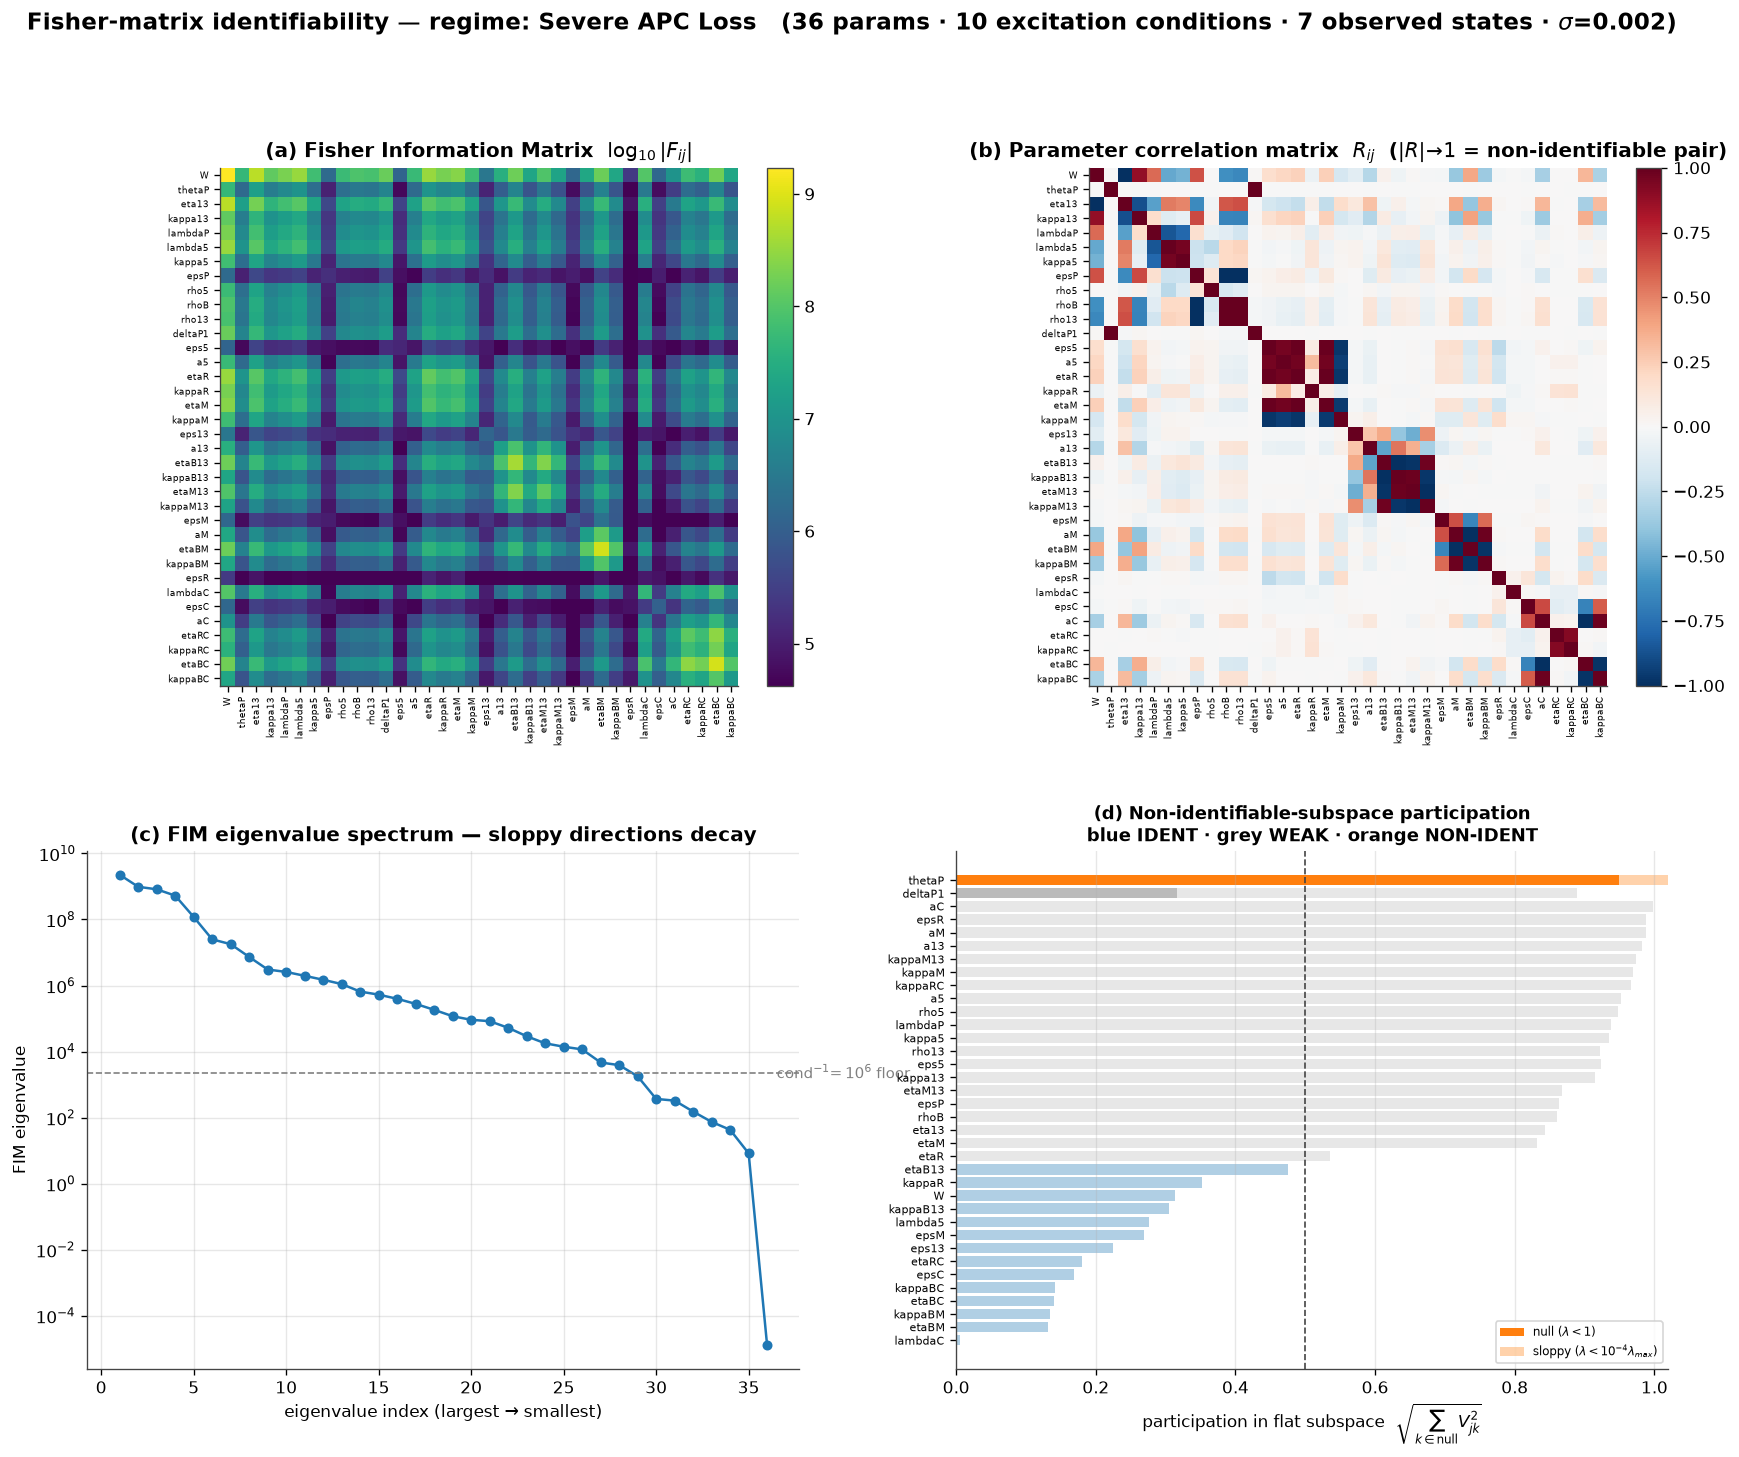
\includegraphics[width=\linewidth]{fim_severe_full36.png}
    \caption{Fisher analysis of the Severe APC Loss regime, full 36-parameter
    problem: (a) magnitude of the information matrix, (b) the parameter
    correlation matrix, (c) the eigenvalue spectrum on a logarithmic axis, and
    (d) each parameter's participation in the flat subspace, colored by
    verdict. The long tail in panel (c) and the off-diagonal blocks in panel
    (b) are the sloppiness and the compensating pairs respectively.}
    \label{fig:fimfull}
\end{figure}

\subsection{A well-posed reduced parameter set}

If the difficulty is a property of the 36-parameter problem rather than of the
model or the data, then restricting to the parameters the data actually
constrain should give a well-posed problem. We tested this by selecting the
eight parameters with the lowest flat-subspace participation across all regimes
--- $\lambda_C$, $\eta_{BM}$, $\kappa_{BM}$, $\kappa_{BC}$, $\eta_{BC}$,
$\eta_{RC}$, $\kappa_{B13}$, $\kappa_R$ --- fixing the other 28 at their true
values, and recomputing the Fisher matrix on identical data. The result is
Table~\ref{tab:fimtop8}.

\begin{table}[H]
\centering
\begin{tabular}{lrccc}
\toprule
\textbf{Regime} & $\mathrm{cond}(F)$ & \textbf{null} & \textbf{sloppy} &
\textbf{verdict} \\
\midrule
Normal            & 99.7  & 0 & 0 & 8/8 identifiable \\
Early Adenoma     & 120.9 & 0 & 0 & 8/8 identifiable \\
Advanced Adenoma  & 229.4 & 0 & 0 & 8/8 identifiable \\
Severe APC Loss   & 665.2 & 0 & 0 & 8/8 identifiable \\
\bottomrule
\end{tabular}
\caption{The eight-parameter subproblem on identical data. The condition number
falls from $10^{7}$--$10^{19}$ to $10^{2}$--$10^{3}$, with no null directions,
no sloppy directions, and no correlated pairs in any regime.}
\label{tab:fimtop8}
\end{table}

The contrast is stark: fifteen to seventeen orders of magnitude of conditioning
recovered by removing 28 parameters. It also shows that the data are not
impoverished in any absolute sense --- they contain enough information to
determine eight parameters comfortably in every regime, including the worst.
The problem is that we were asking them to determine 36. Note also that the
residual regime ordering survives even here: the condition number still climbs
from 99.7 to 665.2 across the progression. The wall is attenuated, not
eliminated, by reducing the parameter set. Figure~\ref{fig:fimcontrast} places
the full and reduced spectra side by side.

\begin{figure}[H]
    \centering
    \begin{subfigure}{0.49\textwidth}
        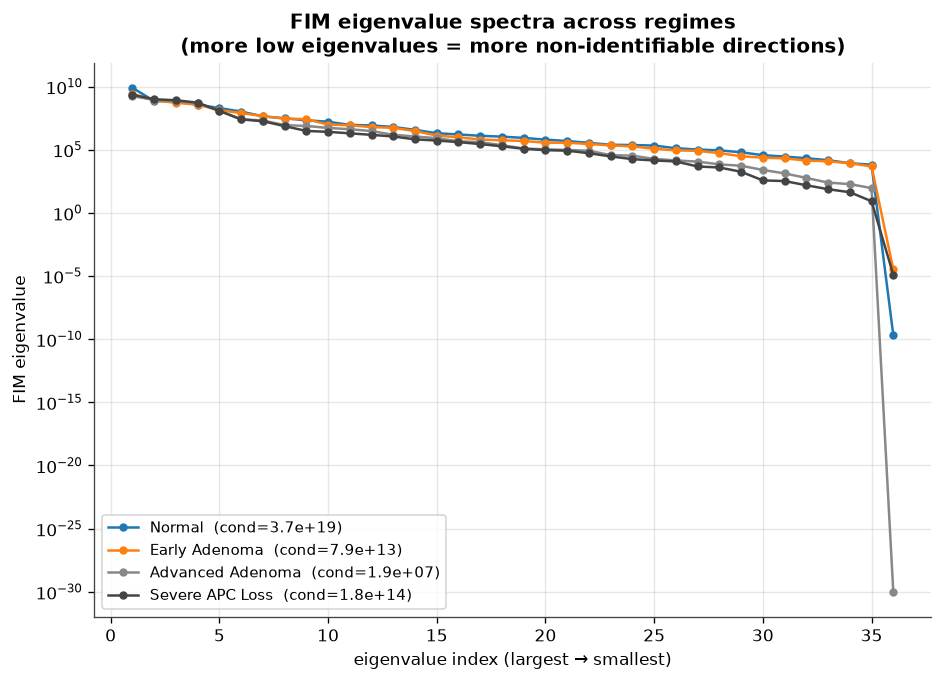
\includegraphics[width=\linewidth]{fim_cross_regime_spectra.png}
        \caption{Spectra across regimes, 36 parameters}
    \end{subfigure}\hfill
    \begin{subfigure}{0.49\textwidth}
        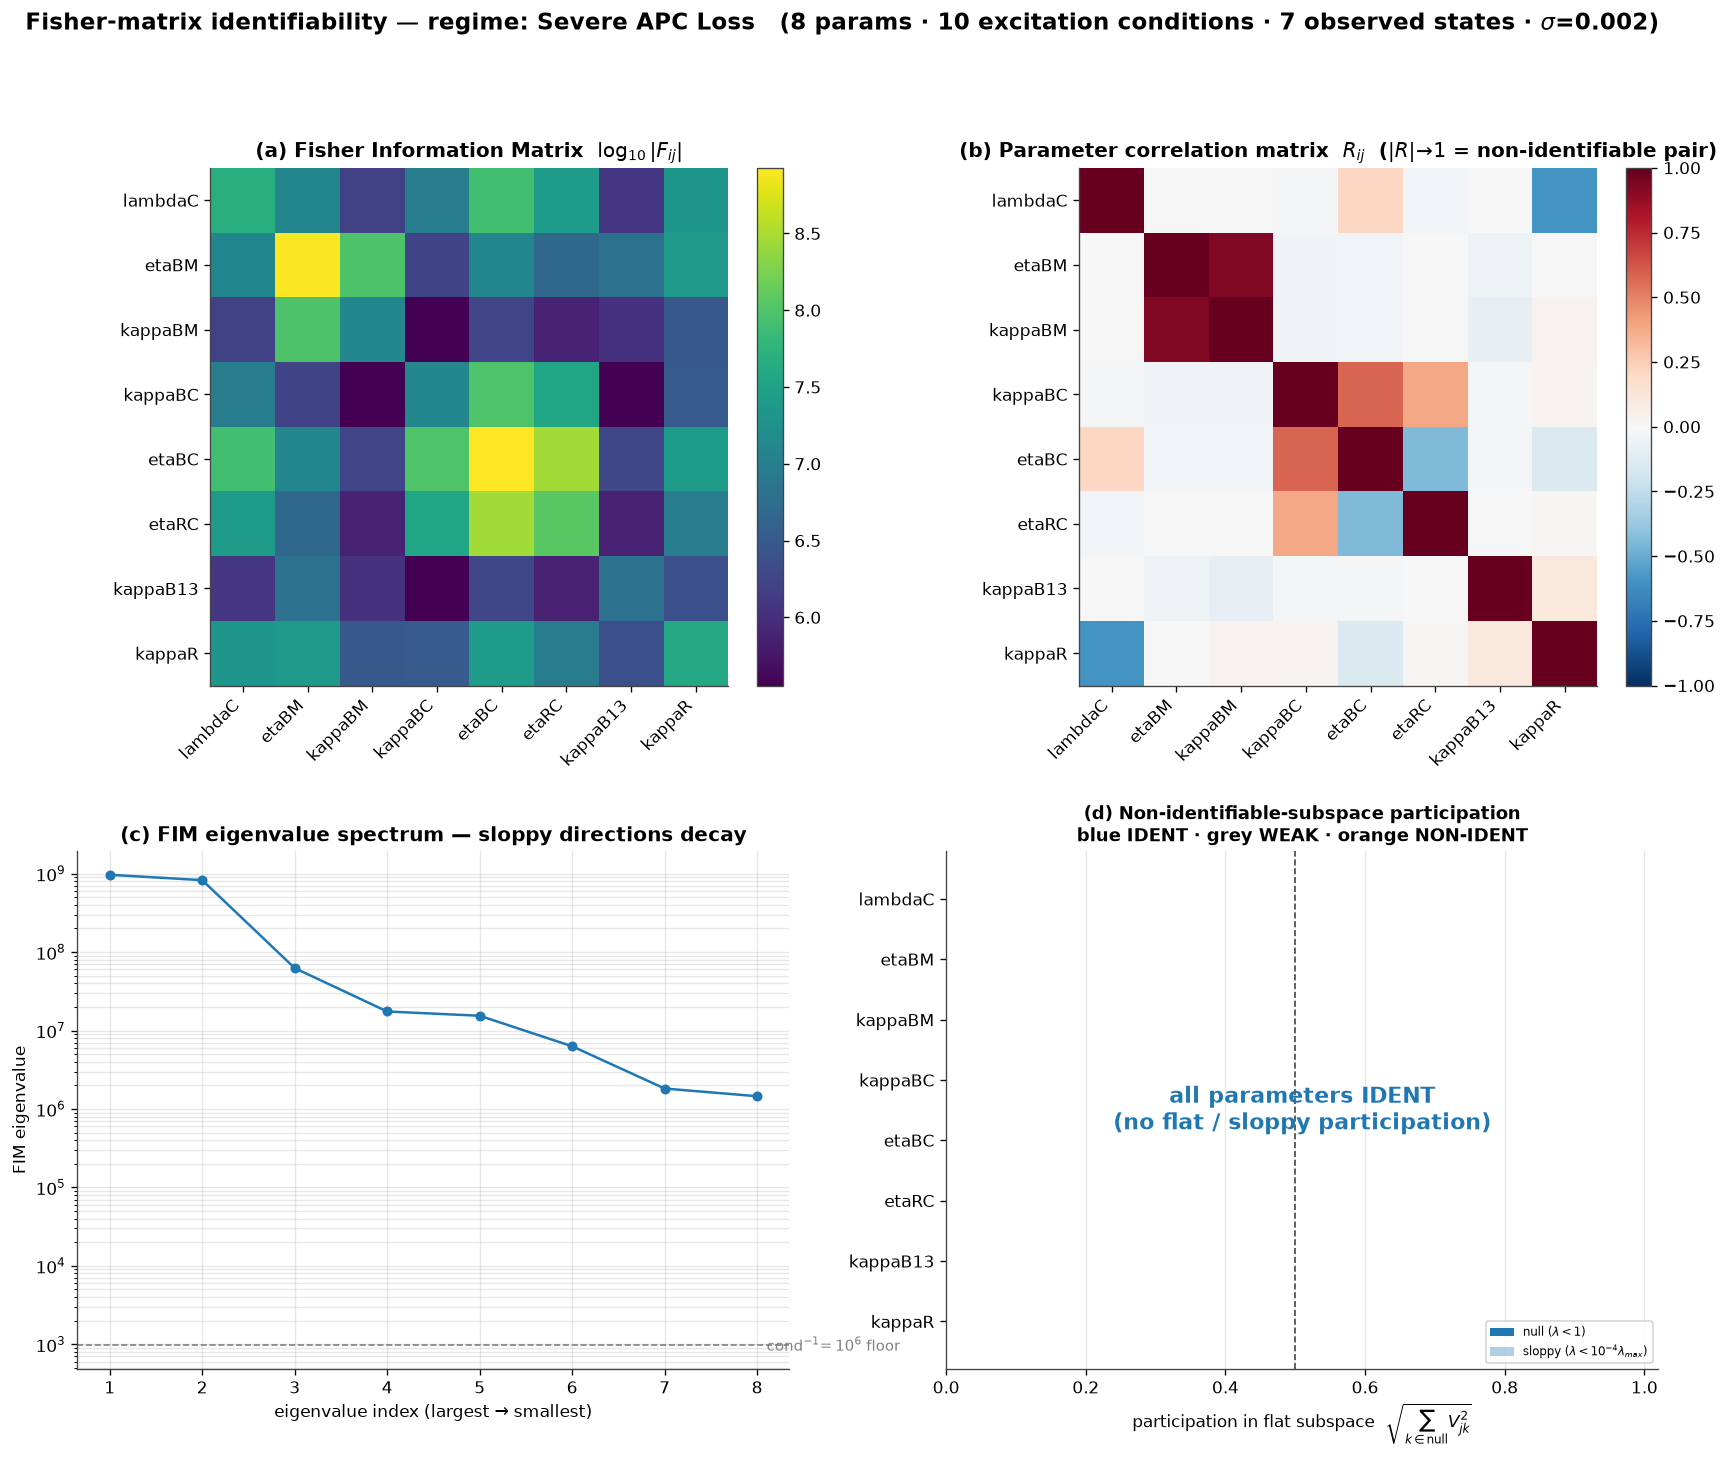
\includegraphics[width=\linewidth]{fim_severe_top8.png}
        \caption{The 8-parameter subproblem, Severe APC Loss}
    \end{subfigure}
    \caption{Left: eigenvalue spectra of the full 36-parameter information
    matrix for all four regimes on a common logarithmic axis, showing the long
    soft tail in each. Right: the same analysis restricted to the eight
    best-constrained parameters in the worst regime --- a compact spectrum, no
    flat directions, and all eight parameters identifiable.}
    \label{fig:fimcontrast}
\end{figure}

\subsection{Profile-likelihood confidence intervals}

The Fisher matrix is a local, quadratic approximation evaluated at the true
parameters. Profile likelihood~\citep{raue2009identifiability} makes no such
approximation: each parameter is scanned over a wide range while all others are
re-optimized at every point, and the confidence interval is read off where the
profile crosses a $\chi^2$ threshold. It is the more trustworthy of the two and
far more expensive.

Starting from the exciting-conditions ODE-fit optimum, we obtained
\textbf{20 identifiable, 16 weak, and 0 strictly non-identifiable} parameters of
36 at the 95\% level, with a 25-fold logarithmic scan window. The agreement with
the Fisher analysis is close and, importantly, independent of it. The
tightest intervals belong to $\varepsilon_M$ (relative width $0.031$;
$[0.596, 0.614]$ against a true $0.60$), $\varepsilon_{13}$ ($0.053$),
$\varepsilon_R$ ($0.060$), and $\lambda_P$ ($0.073$; $[1.576, 1.692]$ against a
true $1.60$). The widest belong to $\eta_R$ ($2.336$), $\eta_{M13}$ ($2.279$),
and $\delta_{P1}$ ($2.144$; $[4.41, 16.12]$ against a true $3.50$), with $W$ at
$0.862$ and $\thP$ at $0.800$, the latter with an interval of $[0.157, 0.785]$
against a true value of $0.50$.

The parameters with the widest profiles are exactly the ones the Fisher matrix
flags as near-degenerate pairs: $\thP$ with $\delta_{P1}$, and $\eta_R$ with
$\eta_M$. Two methods with entirely different assumptions --- one a local
quadratic expansion at the truth, the other a global re-optimized scan from an
estimated optimum --- identify the same pairs. That is the strongest evidence
available here that the degeneracy is real and not an artifact of either
diagnostic.

We must state a limitation squarely: the profile-likelihood analysis completed
for \textbf{one regime only} (Advanced Adenoma). The remaining three reached the
optimization stage and did not finish the profiling within the compute budget,
so no confidence intervals were written for them. We therefore do not claim a
four-regime profile-likelihood analysis, and the numbers above should be read
as a single-regime corroboration of the Fisher result rather than an
independent four-regime replication.

All 36 profiles are reproduced in Figures~\ref{fig:profile}--\ref{fig:profile3},
split across three pages for legibility.

\begin{figure}[H]
    \centering
    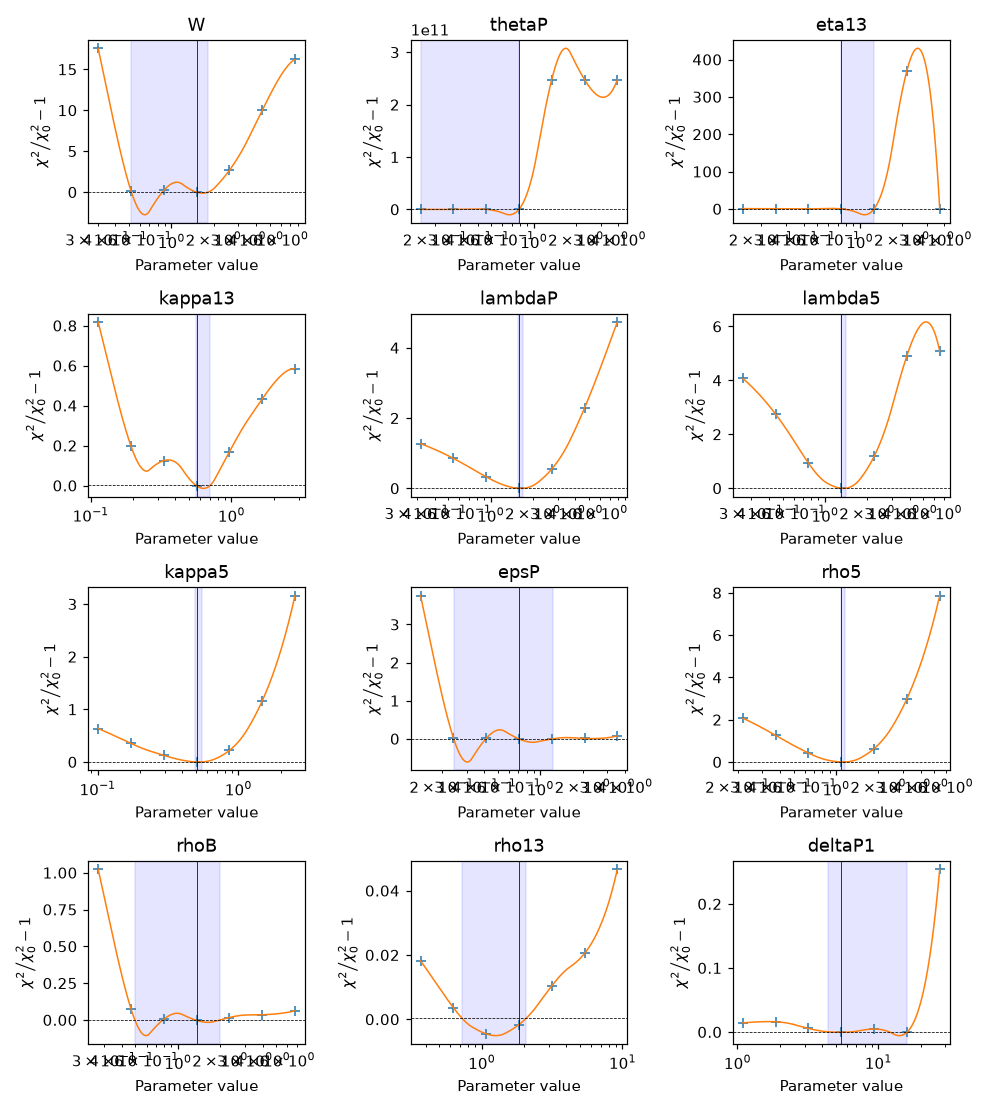
\includegraphics[width=0.95\linewidth,
                     height=0.72\textheight,
                     keepaspectratio]{profile_likelihood_advanced_p1.png}
    \caption{Profile likelihood for the Advanced Adenoma regime, parameters
    1--12 of 36. Each panel scans one parameter while re-optimizing the other
    35; the horizontal line is the 95\% $\chi^2$ threshold. Narrow, sharply
    curved profiles are identifiable parameters; flat or one-sided profiles
    indicate parameters the data cannot pin down. Continued in
    Figures~\ref{fig:profile2} and~\ref{fig:profile3}.}
    \label{fig:profile}
\end{figure}

\begin{figure}[H]
    \centering
    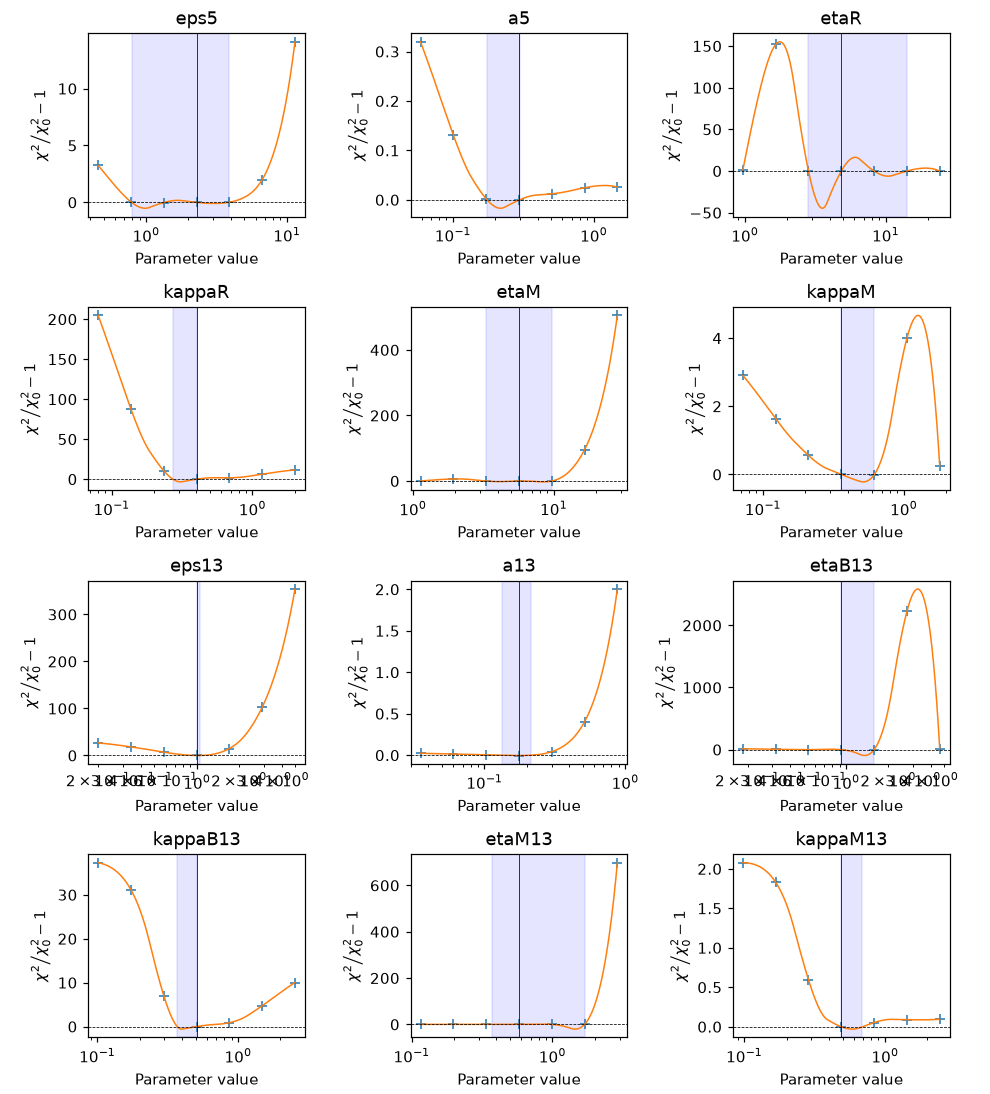
\includegraphics[width=0.95\linewidth,
                     height=0.72\textheight,
                     keepaspectratio]{profile_likelihood_advanced_p2.png}
    \caption{Profile likelihood for the Advanced Adenoma regime, parameters
    13--24 of 36. Axes and thresholds as in Figure~\ref{fig:profile}.}
    \label{fig:profile2}
\end{figure}

\begin{figure}[H]
    \centering
    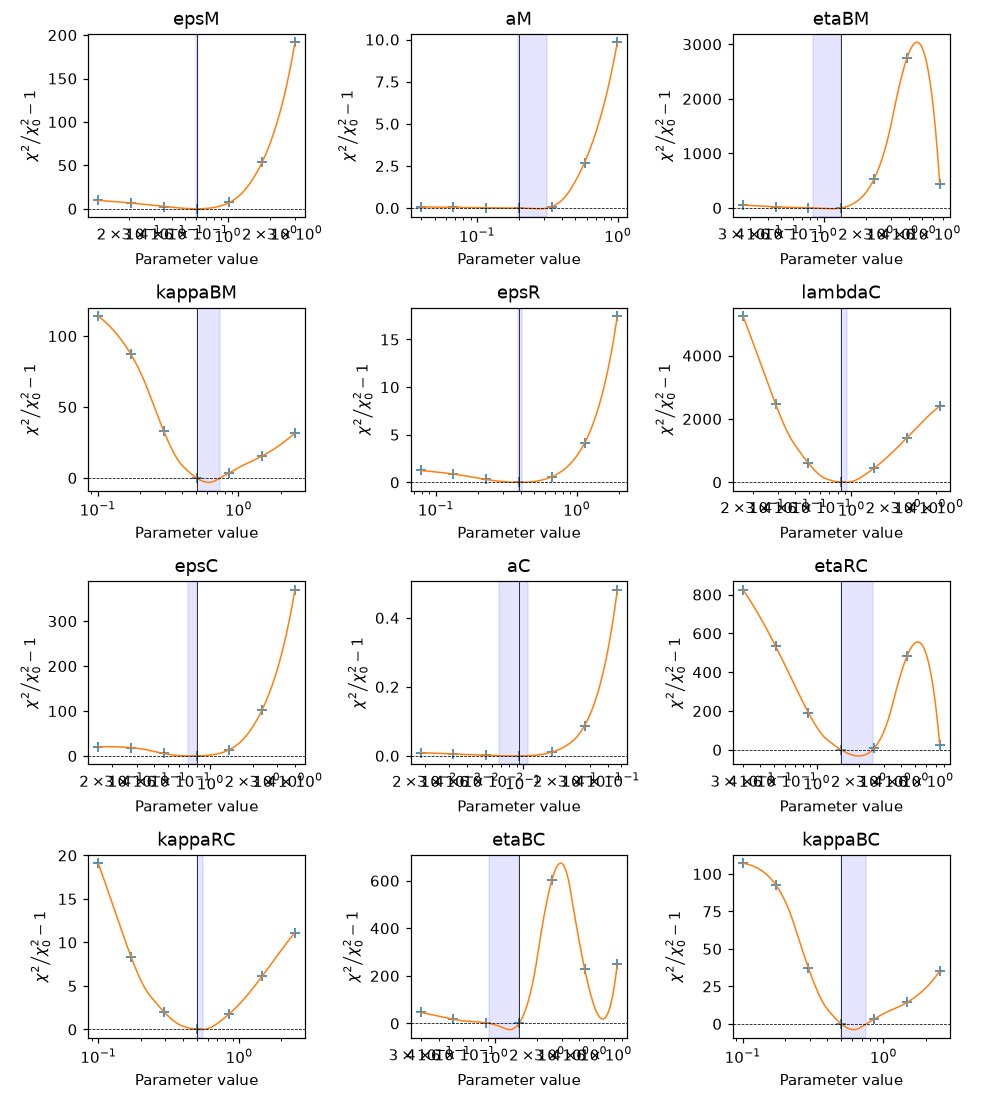
\includegraphics[width=0.95\linewidth,
                     height=0.72\textheight,
                     keepaspectratio]{profile_likelihood_advanced_p3.png}
    \caption{Profile likelihood for the Advanced Adenoma regime, parameters
    25--36 of 36. Axes and thresholds as in Figure~\ref{fig:profile}.}
    \label{fig:profile3}
\end{figure}

\subsection{Consensus verdict}

The evidence converges. An analytic argument shows that $\thP$ and
$\delta_{P1}$ are determined only through their product. The Fisher matrix finds
that degeneracy in every regime without being told, and finds the number of
additional near-degenerate pairs growing $0 \to 1 \to 6 \to 10$ with WNT drive.
Profile likelihood, from a different starting point and with no quadratic
approximation, assigns the widest confidence intervals to the same parameters.
And the inverse runs of Section~\ref{sec:inverse}, using no identifiability
machinery at all, recover $\thP$ in only 5 of 28 attempts and degrade
monotonically across the same ordering.

The mechanism is the one anticipated in Section~\ref{sec:model}. Increasing $W$
drives \bcat{} into saturation of the Hill terms that read it; in that limit the
APC subsystem becomes insensitive to how much APC functionality remains, and
$\thP$ decouples from the observables. The degeneracy is therefore a
conditioning failure created by the operating point, not a flaw in the model
structure --- which is why the de-saturating $D_W = -0.7$ condition of
Section~\ref{sec:inverse} improves matters (recovering $\thP$ to 0.9\% in the
Normal regime) without eliminating the problem in the most extreme regime.
\section{Bayesian inference and posterior calibration}
\label{sec:bayes}

Everything reported so far is a point estimate accompanied by an
\emph{ad hoc} identifiability verdict --- a parameter is called recovered if
its relative error falls below a threshold. A Bayesian treatment replaces this
with a posterior, from which credible intervals and a principled
identifiability statement follow directly: a marginal that has collapsed
relative to its prior is informed by the data, and one that has reverted to the
prior is not~\citep{yang2021bpinns}. We implemented both halves of this: a
Bayesian \emph{inverse} PINN, sampling the parameters with the state networks
frozen, and a Bayesian \emph{forward} PINN, sampling the network weights with
the parameters known.

We report this section in an unusual amount of detail because our first
inverse run failed in a way that is instructive, generic to Bayesian PINNs, and
--- in our reading of the literature --- not adequately flagged. It produced
posteriors that were simultaneously extremely confident and badly wrong, and
the naive identifiability verdict computed from them declared all 36 parameters
identifiable in all four regimes.

\subsection{Sampler and priors}

Both analyses use Hamiltonian Monte Carlo~\citep{neal2011mcmc}, which is the
appropriate sampler here: gradients of the log posterior are available by
automatic differentiation at no extra cost, and HMC's efficiency degrades far
more gracefully with dimension than random-walk Metropolis or variational
approximations. Our implementation is a static-path HMC with a dense mass
matrix rather than NUTS. The mass matrix is initialized from the Laplace
approximation at the MAP --- the Hessian of the potential, eigenvalue-floored
to guarantee positive definiteness --- and then re-adapted from the warmup
sample covariance. The step size is set by the standard heuristic search
followed by dual averaging to a target acceptance rate of
$0.8$~\citep{hoffman2014nuts}, and the trajectory length is jittered by
$\pm 3$ leapfrog steps per draw to avoid resonances. Non-finite Hamiltonians
are hard-rejected as divergences.

Sampling is performed in the unconstrained space in which the parameters are
represented: 35 of the 36 are sampled in log space and $\thP$ in logit space,
so positivity and the $(0,1)$ constraint on $\thP$ are enforced by
construction. The priors are Gaussian in that space, with $\sigma_{\text{prior}}
= 1.0$ on the log parameters and $\sigma_{\text{prior}} = 2.0$ on the logit of
$\thP$, the latter being close to flat on $(0,1)$. Chains are initialized at
the integral-residual MAP estimate of Section~\ref{sec:integral}.

We note one limitation up front: each regime is sampled with a single chain, so
no $\hat{R}$ diagnostic is available. Mixing is assessed by effective sample
size alone, computed by Geyer's initial-monotone-sequence truncation.

\subsection{Likelihood specification and a calibration failure}
\label{sec:bayesfail}

Because the state networks are frozen, the data term is constant in $\theta$
and drops out of the posterior; the only $\theta$-dependent term is the physics
residual. The first implementation took the obvious route and treated every
residual evaluation as an independent observation:
\begin{equation}
U(\theta) = \frac{1}{2\sigma_{\text{res}}^2}
\sum_{i=1}^{N_{\text{res}}} r_i(\theta)^2
+ \sum_j \frac{s_j^2}{2\sigma_{\text{prior},j}^2},
\label{eq:badpotential}
\end{equation}
with $\sigma_{\text{res}}$ calibrated so that the reduced $\chi^2$ equals one
at the MAP, i.e. $\sigma_{\text{res}} = \sqrt{\mathrm{SSR}_{\mathrm{MAP}} /
N_{\text{res}}}$.

The trouble is $N_{\text{res}}$. With 10 conditions, 7 states, and 3000
collocation points, $N_{\text{res}} = 209{,}930$, and $\sigma_{\text{res}}$
calibrates to $\sim\!5\times10^{-4}$. Nothing in Eq.~\eqref{eq:badpotential}
knows that adjacent collocation points on a smooth trajectory carry almost no
independent information. The posterior precision therefore scales with the
\emph{density of the collocation grid} rather than with the information content
of the experiment: refine the grid and the posterior tightens, without a single
new measurement having been made. The potential energy sits around
$U \approx 8.7\times 10^{4}$, and the resulting posterior is a needle.

The consequences are recorded in Table~\ref{tab:bayesfail}. Effective sample
sizes are 3--6 out of 1500 draws, so the chain is not mixing at all; the
posterior mean sits a median of 29--51 standard deviations from the truth,
with worst cases in the hundreds; and the 95\% credible interval covers the
true value for at most 1 of 36 parameters in any regime. Individual cases make
the failure vivid. In the Severe APC Loss regime the posterior for $W$ is
$1.1203 \pm 0.0043$ against a true value of $2.00$ --- a $z$-score of $-206$
--- while $\thP$ is $0.6134 \pm 0.0011$ against a true $0.25$, a $z$-score of
$+332$.

\begin{table}[H]
\centering
\small
\setlength{\tabcolsep}{5pt}
\begin{tabular}{lccccc}
\toprule
\textbf{Regime} & \textbf{median ESS} & \textbf{median $|z|$} &
\textbf{max $|z|$} & \textbf{CI$_{95}$ coverage} &
\textbf{reported verdict} \\
\midrule
Normal            & 3.4 & 38.4 & 784 & 1/36 & 36/36 IDENT \\
Early Adenoma     & 5.6 & 29.0 & 466 & 0/36 & 36/36 IDENT \\
Advanced Adenoma  & 3.1 & 50.1 & 293 & 1/36 & 36/36 IDENT \\
Severe APC Loss   & 5.4 & 50.9 & 563 & 1/36 & 36/36 IDENT \\
\bottomrule
\end{tabular}
\caption{The miscalibrated first run. $z = (\text{posterior mean} -
\text{truth})/\text{posterior std}$; ESS is out of 1500 draws. Every diagnostic
that was actually computed at the time (posterior width) looked excellent;
every diagnostic that was not (mixing, coverage) was catastrophic.}
\label{tab:bayesfail}
\end{table}

The last column is the important one. The identifiability verdict was computed
purely as \emph{shrinkage relative to the prior},
\begin{equation}
\mathrm{shrink}_j = \frac{\mathrm{std}(s_j \mid \mathcal{D})}
{\sigma_{\text{prior},j}},
\qquad
\begin{cases}
\text{IDENT} & \mathrm{shrink} < 0.30,\\
\text{WEAK} & 0.30 \le \mathrm{shrink} < 0.70,\\
\text{NON-IDENT} & \text{otherwise},
\end{cases}
\label{eq:shrink}
\end{equation}
and these posteriors were \emph{tight but biased}, with
$\mathrm{shrink}(W)$ in the range $0.0006$--$0.0038$. A width-based criterion
reads that as maximal information. The general lesson is that in a Bayesian
PINN, posterior width is not evidence of identifiability unless the sampler is
mixing and the intervals are calibrated; a physics likelihood summed over a
dense collocation grid can manufacture arbitrarily small credible intervals
around an arbitrarily wrong answer.

\subsection{The corrected likelihood and its effect}

The fix is to stop pretending that $2\times10^5$ correlated residual
evaluations constitute $2\times10^5$ independent observations. We rescale the
physics term by a fixed effective sample size:
\begin{equation}
U(\theta) = \frac{n_{\text{eff}}}{N_{\text{res}}}\cdot
\frac{1}{2\sigma_{\text{res}}^2}\sum_{i=1}^{N_{\text{res}}} r_i(\theta)^2
+ \sum_j \frac{s_j^2}{2\sigma_{\text{prior},j}^2},
\qquad
n_{\text{eff}} = n_{\text{cond}} \times 7 \times n_{\text{obs}},
\label{eq:goodpotential}
\end{equation}
where $n_{\text{obs}} = 40$ is the actual per-trajectory observation budget of
the sparse-data setting. With 10 conditions this gives $n_{\text{eff}} = 2800$
against $N_{\text{res}} = 279{,}930$, a downweighting of roughly $100\times$,
and --- the point of the construction --- a posterior width that no longer
depends on how finely the collocation grid is drawn. Written this way the
physics term is an $n_{\text{eff}}$-weighted \emph{mean} residual rather than a
sum, and $\sigma_{\text{res}}$ (still the per-point RMS residual at the MAP)
becomes orthogonal to the sample-size choice instead of fighting it.

We additionally gate reporting on two diagnostics that would have caught the
original failure: a regime's verdicts are reportable only if the median ESS is
at least 200 \emph{and} the credible intervals cover the truth for at least
33 of 36 parameters. Table~\ref{tab:bayesfixed} gives the corrected run.

\begin{table}[H]
\centering
\begin{tabular}{lccccc}
\toprule
\textbf{Regime} & \textbf{ESS (median)} & \textbf{median $|z|$} &
\textbf{covers truth} & \textbf{accept} & \textbf{gate} \\
\midrule
Normal            & 96   & 1.3 & 21/36 & 0.79 & fail \\
Early Adenoma     & 1265 & 1.6 & 20/36 & 0.68 & fail \\
Advanced Adenoma  & 12   & 5.8 &  8/36 & 0.70 & fail \\
Severe APC Loss   & 15   & 9.9 &  9/36 & 0.67 & fail \\
\bottomrule
\end{tabular}
\caption{The corrected run (3000 warmup, 3000 draws, 48 leapfrog steps). The
posteriors are now approximately honest --- median $|z|$ has fallen from
29--51 to 1.3--9.9 --- but the gate still fails in all four regimes, so we do
not report IDENT/NON-IDENT counts from them.}
\label{tab:bayesfixed}
\end{table}

We emphasize what this table does and does not license. The median $|z|$ has
fallen by more than an order of magnitude, from 29--51 to 1.3--9.9, so the
posteriors are no longer confidently wrong. But no regime passes the gate, so
we do not quote a Bayesian identifiability count as a result. What the table
does support is a calibration-based restatement of the $\thP$ wall that is
independent of any threshold: coverage degrades monotonically with WNT drive,
21/36 $\to$ 20/36 $\to$ 8/36 $\to$ 9/36, and the median $|z|$ climbs
monotonically, $1.3 \to 1.6 \to 5.8 \to 9.9$. The posterior becomes
progressively less able to bracket the truth exactly as the system moves into
the high-WNT regimes, which is what Sections~\ref{sec:inverse}
and~\ref{sec:ident} predict from entirely different evidence.

Scored the same way as every other estimator in this paper --- posterior mean
within 10\% relative error --- the corrected posteriors recover
\textbf{19/20/11/8} parameters across the four regimes. That is at most a few
parameters better than the integral-residual point estimate that seeded the
chains (17/16/10/7), and it does not clear the ceiling established in
Section~\ref{sec:inverse}. This is the honest headline for the Bayesian inverse
work: it upgrades point estimates to intervals and exposes the calibration
question, but it does not by itself recover more of the model.

\subsection{Posterior-predictive uncertainty in the forward problem}

The forward twin holds the parameters fixed and samples the network weights, so
the posterior-predictive spread is uncertainty about the \emph{solution} given
sparse noisy observations. This is a harder sampling problem in the trivial
sense --- the state of the chain is 10,951 network weights rather than 36
parameters --- which forces a diagonal mass matrix, but an easier one in the
sense that we only care about a low-dimensional functional of the weights.

The setup uses 40 noisy observations at $\sigma = 0.02$, 800 collocation
points, 1000 warmup and 1000 draws at 40 leapfrog steps, with a
$\mathcal{N}(0, 3^2)$ prior on the weights and three likelihood terms (data,
initial condition, physics), each with its scale calibrated to the
corresponding residual at an Adam-trained MAP. A useful self-consistency check
falls out of that calibration: the data noise scale recovers as
$\sigma_{\text{data}} = 1.952\times10^{-2}$ against the true injected
$0.02$.

The first attempt under-covered badly, at mean 95\% coverage of
$0.73/0.63/0.63/0.56$ across the four regimes, because it reported only the
\emph{epistemic} band --- the spread of the posterior mean function --- and
compared it against \emph{noisy} observations. The correct comparison adds the
observation noise back,
$\sigma_{\text{pred}}^2 = \sigma_{\text{epi}}^2 + \sigma^2$, giving the
posterior predictive rather than the posterior mean band. With that correction
the two bands separate cleanly and both are calibrated
(Table~\ref{tab:fwdbayes}): the epistemic band is 0.3--0.6\% of state scale and
covers the noise-free truth 91--96\% of the time, while the predictive band is
6.7--8.0\% of state scale and covers the noisy observations 94--95\% of the
time.

\begin{table}[H]
\centering
\small
\setlength{\tabcolsep}{5pt}
\begin{tabular}{lcccc}
\toprule
\textbf{Regime} & \textbf{predictive} & \textbf{rel. predictive} &
\textbf{epistemic} & \textbf{rel. epistemic} \\
& \textbf{coverage} & \textbf{width} & \textbf{coverage} & \textbf{width} \\
\midrule
Normal           & 0.95 & 0.080 & 0.96 & 0.006 \\
Early Adenoma    & 0.94 & 0.073 & 0.91 & 0.004 \\
Advanced Adenoma & 0.94 & 0.069 & 0.96 & 0.003 \\
Severe APC Loss  & 0.95 & 0.067 & 0.96 & 0.003 \\
\bottomrule
\end{tabular}
\caption{Bayesian forward PINN. Predictive coverage is against the noisy
observations; epistemic coverage is against the noise-free reference. Band
widths are relative to state scale. Mean relative RMSE against the reference is
0.001--0.002 in all regimes.}
\label{tab:fwdbayes}
\end{table}

The separation between the two bands is visible directly in
Figure~\ref{fig:fwdbands}.

\begin{figure}[H]
    \centering
    
\includegraphics[width=\linewidth]{fwd_beta_bands.png}
    \caption{Posterior-predictive bands for \bcat{} across the four regimes.
    Each panel shows the wide 95\% posterior-predictive band, the narrow 95\%
    reconstruction (epistemic) band, the posterior mean, the noise-free
    reference, and the 40 noisy observations. The predictive band is dominated
    by the observation noise; the epistemic band, which is what the network
    itself is uncertain about, is roughly an order of magnitude narrower.}
    \label{fig:fwdbands}
\end{figure}

Two caveats are worth recording. First, coverage is scored against the same 40
points that entered the data likelihood, so it is an in-sample calibration
check, not a held-out one. Second, the ESS of the potential energy itself is
3--4, meaning the weight-space chain is emphatically not mixed; what mixes is
the low-dimensional predictive functional, whose ESS is 97--400. The band is
therefore trustworthy as a statement about the predicted trajectory and should
not be read as a converged exploration of weight space. This is a common
situation in Bayesian deep learning and is one reason posterior-predictive
quantities are the right thing to report.
\section{Discussion}
\label{sec:discussion}

\subsection{Principal findings}

Read as a whole, the experiments make one argument. For a model of this class,
the quantity that limits parameter recovery is the information content of the
experiment, and almost nothing else we tried was a substitute for it.

The evidence for that claim is largely negative, which is what makes it
credible. Shrinking the network by a factor of five and regularizing it made
recovery slightly worse. Alternating two-timescale optimization made it
slightly worse. Adding a Stage-3 parameter refinement made no difference.
Tripling the number of experimental conditions, when the new conditions
perturbed the same input as the old ones, moved recovery from 5 to 7 of 36
while making the estimate of $W$ monotonically worse. Only two interventions
produced large gains, and both changed what the estimator was fitting rather
than how it searched: replacing the differentiated residual with an integral
one ($+13$ parameters at fixed conditions), and adding perturbation channels
that reach the network through new doors ($+21$ for the classical estimator).

The second of these is the more general lesson, and it is essentially a
statement about experimental design. Our first six conditions were all
variations of the ATRA protocol, and every one of them entered the WNT/HOX/MYC
subnetwork through the single term $\eta_R r/(\kappa_R+r)$. No amount of
reshaping a signal that passes through one door will separate the parameters
behind it. Four conditions that drive \bcat{} and MYC directly were worth more
than any number of the former, and the single most targeted of them --- a
sustained WNT-inhibiting step designed to pull \bcat{} out of saturation ---
recovered $\thP$ to within 0.9\% in the regime where it had previously failed.
Designing the perturbation to break a specific degeneracy is a different and
more productive activity than collecting more data.

\subsection{Methodological implications for physics-informed neural networks}

Two findings concern the PINN formulation specifically, and we think both
generalize beyond this model.

\textbf{The autodiff residual is a biased estimator of the parameters.} The
strong-form residual $\dot z_\phi - f(z_\phi;\theta)$ requires the network's
time derivative, and a network can fit a trajectory well while its derivative is
noticeably wrong. Any such error is absorbed by $\theta$. Our controlled
experiment made the consequence explicit: minimizing the residual to
$2.39\times10^{-4}$ --- a factor of 1550 below the joint-training value --- put
$W$ at 37\% error, worse than the joint run achieved at a far higher residual.
Lower loss, worse parameters. The integral form of Eq.~\eqref{eq:integral}
avoids forming the derivative at all and recovers roughly half the gap to the
classical estimator. Because published PINN inverse results are almost
universally reported with the strong-form residual, this seems worth flagging
as a systematic concern rather than a quirk of our system.

The same phenomenon reappeared where we did not expect it, in model selection.
Choosing between two restarts by their final physics residual picked the
worse-recovering restart in three of four regimes; the better-recovering
choices would have yielded 55 rather than 50 parameters. If residual value does
not rank two fits of the same model correctly, it should not be used as a
selection criterion for inverse problems.

\textbf{Posterior width is not evidence of identifiability.} Our Bayesian
inverse PINN initially reported all 36 parameters as identifiable in all four
regimes, on the basis of posteriors that had collapsed to a small fraction of
their priors. Those posteriors excluded the truth by a median of 29--51
standard deviations, with effective sample sizes of 3 to 6 out of 1500 draws.
The cause was treating $2.1\times10^{5}$ correlated residual evaluations on a
dense collocation grid as independent observations, which makes posterior
precision a function of grid density rather than of information. Because the
verdict criterion measured only shrinkage relative to the prior, a tight-and-wrong
posterior read as maximal information.

We suspect this failure is common and under-reported, for a structural reason:
a Bayesian PINN's physics likelihood has no natural sample size, the number of
collocation points is chosen for numerical accuracy rather than statistical
reasons, and the diagnostic that would catch the problem (interval coverage
against known truth) is unavailable in the applied setting where the truth is
unknown. Our mitigation --- rescaling the physics term by a fixed effective
sample size tied to the real observation budget --- restores grid-independence
and brought the median discrepancy down from 29--51 to 1.3--9.9 standard
deviations. It did not, however, produce chains that pass our own mixing and
coverage gate, so we report no Bayesian identifiability counts. We would rather
report a gate that fails than a number that looks clean.

\subsection{Biological interpretation}

Within the limits of an idealized model fitted to synthetic data, two results
have biological content.

The forward solutions predict a \textbf{progressive loss of ATRA
responsiveness} along the adenoma--carcinoma sequence, and they predict it
unevenly across species. HOXA5 responds strongly to treatment in all four
regimes, but HOXA13 barely falls at all in Advanced Adenoma and Severe APC
Loss, and APC becomes markedly less responsive because the elevated degradation
$\delta_P(\thP)$ caps the level it can reach regardless of how much HOXA5 is
induced. The differentiation signal still arrives; the machinery that would
translate it into suppression of the proliferative program no longer can. This
emerges from the network structure rather than being imposed, and it is
consistent with the clinical observation that retinoid monotherapy has been far
more successful in acute promyelocytic
leukemia~\citep{degos2001atra} than in solid tumors of the colon.

The sensitivity analysis places \textbf{APC functionality among the most
influential parameters}, with each state otherwise governed by its own pathway
driver. Locally it dominates outright, with an elasticity of $-3.61$ on
stemness against $1.04$ for the runner-up; measured as a variance share over a
range it sits in a leading cluster with the HOXA13$\to$\bcat{} and
RA$\to$HOXA5 arms rather than standing alone. Either way its prominence is
consistent with APC loss being the initiating event of the
sequence~\citep{fearon1990genetic,kinzler1996hereditary}.
The uncomfortable corollary is the one this paper spends most of its length on:
the single most influential parameter in the model is also among the least
recoverable, recovering in 5 of 28 attempts, precisely because the regimes in
which it matters most are the regimes in which \bcat{} saturation hides it.

\subsection{Limitations}

We are working with synthetic data generated from the model itself, with
Gaussian noise and all seven states observed. Real measurements would be
partial, sparser, differently distributed, and subject to model misspecification
of a kind entirely absent here. Every recovery count in this paper should
therefore be read as an upper bound.

The parameter values are one internally consistent realization rather than a
set fitted to experimental data, so the model is a testbed for methodology and
not a calibrated predictive instrument. Its predictions about ATRA
responsiveness are qualitative.

On the computational side, several limitations are worth naming. All runs use a
single seed, so we report no seed-to-seed variability and no error bars on any
count. The ablation that would separate the integral residual from its three
accompanying changes did not complete, so that gain is attributed to the bundle.
The profile-likelihood analysis completed for one regime of four. The Bayesian
chains are single-chain, so no $\hat{R}$ diagnostic is available, and none passes
our own reporting gate. No symbolic structural identifiability analysis was
performed, so apart from the $(\thP, \delta_{P1})$ lumping every identifiability
claim here is a practical one. And the 27-state sensitivity analysis
mean-imputed roughly 8\% of failed solves, with a Morris nonlinearity flag that
is saturated at that sample size and therefore uninformative.

\subsection{Outlook}

The obvious next step follows from the finding that information is the binding
constraint: rather than adding conditions and checking what improves, use the
Fisher matrix or the profile likelihood to \emph{design} the condition that
maximally reduces uncertainty along a specific degenerate direction. Our
$D_W = -0.7$ de-saturating step was chosen by exactly this reasoning, informally;
formalizing it as optimal experimental design is a natural continuation.

A second direction concerns the Bayesian analysis. The correct effective sample
size for a physics likelihood is not obvious --- ours is a defensible choice,
not a derived one --- and we suspect a principled treatment, perhaps via the
correlation length of the residual field, would be of general use to the B-PINN
literature.

Finally, this paper deliberately holds the model structure fixed and asks only
about its parameters. The complementary question is what happens when part of
the structure is unknown and is replaced by a learned term, as in
neural-mechanistic hybrids and universal differential
equations~\citep{faure2023hybrid,velioglu2025pinn,liu2022hybrid}. That
extension raises its own identifiability questions --- in particular, whether a
learned term absorbs parameters of the equation that hosts it --- and is the
subject of separate work.

\section{Conclusions}
\label{sec:conclusion}

This paper makes two claims, one about a model and one about its approximation.

\textbf{First, we developed a new ODE model of the WNT--RA--HOX axis in
colorectal cancer.} The system couples seven states --- \bcat{}, APC, HOXA5,
HOXA13, MYC, retinoic acid, and CYP26A1 --- through a single elementary
principle, that each species accumulates at the rate at which it is produced
minus the rate at which it is removed (Eq.~\eqref{eq:balance}). Reducing a
27-state reaction network to these seven, and nondimensionalizing, yields 36
dimensionless parameters and a forcing that superimposes circadian dietary
retinoid intake on a smooth ATRA treatment pulse. Four regimes obtained by
raising WNT drive $W$ and lowering APC functionality $\thP$ reproduce the
adenoma--carcinoma sequence, and a derived stemness index provides a single
scalar readout. The model behaves as a model of this system should: a
three-method global sensitivity analysis places APC functionality among the most
influential parameters --- dominant locally, and in a leading cluster of three
when measured as a variance share --- gives each state an interpretable
own-pathway driver, and shows the reduced system to be nearly additive, in
contrast to the strongly interacting network it descends from. Forward solutions
predict a progressive and species-specific loss of ATRA responsiveness along the
sequence, an emergent consequence of the network structure rather than an
imposed assumption.

\textbf{Second, we established that this system can be approximated by neural
networks in both directions.} In the forward direction the approximation is
accurate and cheap in data: a Fourier-feature network reproduces the stiff
\texttt{Radau} reference trajectories to 1--3\% relative error across all four
regimes, and does so from 40 sparse random observations by leaning on the
physics residual, at roughly $2.4\times$ the error of a dense-label fit that
uses $2.5\times$ more data. The multi-timescale retinoid forcing makes the
Fourier embedding mandatory rather than cosmetic: without it the network
recovers under half the treatment-pulse amplitude and none of the circadian
ripple. In the inverse direction the approximation also succeeds, but only up to
a ceiling that we are able to decompose. An estimator defect --- the bias in the
automatic-differentiation residual --- costs 13 parameters and is removed by an
integral residual that never forms the derivative. An information deficit costs
21 more and is addressed only by perturbations that reach the network through
new channels; further experiments of the kind already performed are close to
worthless.

The residue is a genuine limit of the problem rather than of the method, and
four independent analyses agree on where it lies. An analytic argument, the
Fisher information spectrum, profile likelihood, and Bayesian posterior coverage
all show that as WNT drive increases \bcat{} saturates, $\thP$ decouples from
the observables, and the number of near-degenerate parameter pairs grows
$0 \to 1 \to 6 \to 10$. Restricting to the eight best-constrained parameters
gives a well-posed problem with condition number $10^{2}$--$10^{3}$ instead of
$10^{7}$--$10^{19}$, which locates precisely where the recoverable information
lives. The uncomfortable corollary is that the most influential parameter in the
model is among the least recoverable, for the same reason in both cases.

Two cautions accompany these results, and we report them with the same weight as
the successes. The default proportional sampling box of the sensitivity analysis
pushed one parameter past a sign change in the model, producing a variance share
above unity and a plausible-looking but incorrect ranking. And a Bayesian PINN
whose physics likelihood summed over a dense collocation grid produced posteriors
that were extremely confident and badly wrong, certifying all 36 parameters as
identifiable in all four regimes; posterior width is not evidence of
identifiability unless the chain is mixing and the intervals are calibrated. We
believe the second failure mode is generic to Bayesian PINNs and inadequately
flagged in the literature.

Taken together, the model of Section~\ref{sec:model} and the approximation
results that follow it establish that a mechanistic description of WNT--RA--HOX
signaling in colorectal cancer is tractable to physics-informed learning in both
the forward and the inverse direction, and they identify the binding constraint
on what such learning can deliver. That constraint is the information content of
the experiment, not the expressiveness of the network --- which makes
experimental design, rather than architecture search, the productive direction
for work of this kind.

\section*{Data and code availability}

All code, run logs, trained checkpoints, and numeric result tables are in the
project repository. The forward accuracy figures of Table~\ref{tab:fwderr} are
regenerated from saved checkpoints against a fresh \texttt{Radau} reference and
written to \texttt{forward\_error\_table.\{txt,json\}} in each run directory.
The sensitivity tables are written as CSV alongside the figures, in both the
original and the $\thP$-clipped sampling boxes described in
Section~\ref{sec:sa}. Fisher matrices, eigenspectra, correlation matrices and
per-parameter verdicts are saved per regime, as are the profile-likelihood
confidence intervals and all posterior summaries. Every training run records the
random seed, which is fixed at 42 throughout.

\section*{Acknowledgments}

Computations were performed in PyTorch~\citep{paszke2019pytorch} and
SciPy~\citep{virtanen2020scipy}, with sensitivity analysis by
SALib~\citep{herman2017salib}.

\bibliographystyle{unsrtnat}
\bibliography{references}

\end{document}
